%% wheelchart.tex
%% Copyright 2023 Matthias Floré
%
% This work may be distributed and/or modified under the
% conditions of the LaTeX Project Public License, either version 1.3c
% of this license or (at your option) any later version.
% The latest version of this license is in
%   http://www.latex-project.org/lppl.txt
% and version 1.3c or later is part of all distributions of LaTeX
% version 2005/12/01 or later.
%
% This work has the LPPL maintenance status `maintained'.
% 
% The Current Maintainer of this work is Matthias Floré.
%
% This work consists of the files wheelchart.pdf, wheelchart.sty,
% wheelchart.tex and README.md.
\documentclass[a4paper,english,dvipsnames]{ltxdoc}
\usepackage[english]{babel}
\usepackage{graphicx}
\usepackage[a4paper,left=2.25cm,right=2.25cm,top=2.5cm,bottom=2.5cm]{geometry}
\usepackage{parskip}
\usepackage{iftex}
\ifluatex
\else
\usepackage[T1]{fontenc}
\usepackage[utf8]{inputenc}
\fi
\usepackage[page]{totalcount}%\totalpages or \getpagerefnumber{Thesourcecode}-1
\usepackage{mathtools}
\usepackage{amssymb}
\usepackage{interval}
\allowdisplaybreaks
\usepackage{tabularray}
\UseTblrLibrary{counter,siunitx}
\usepackage{listofitems}
\usepackage{pdflscape}
\usepackage{wheelchart}
\usetikzlibrary{decorations.markings,decorations.text,patterns}
\usepackage{tikzlings}
\input{pgfmanual-en-macros.tex}
%The environments commandmeta and commandmetameta and the macros \extractcommandmeta and \extractcommandmetameta below are modified from pgfmanual-en-macros.tex
\newenvironment{commandmeta}[2]{
  \begin{pgfmanualentry}
    \extractcommandmeta#1#2\@@
    \pgfmanualbody
}
{
  \end{pgfmanualentry}
}
\def\extractcommandmeta#1#2\@@{%
  \removeats{#1}%
  \pgfmanualentryheadline{%
    \pgfmanualpdflabel{\textbackslash\strippedat\meta{#2}}{}%
    \declare{\expandafter\texttt\expandafter{\string#1\meta{#2}}}%
  }%
  \index{\strippedat\meta{#2} @\protect\myprintocmmand{\strippedat\meta{#2}}}
}
\newenvironment{commandmetameta}[2]{
  \begin{pgfmanualentry}
    \extractcommandmetameta#1\@@#2\@@
    \pgfmanualbody
}
{
  \end{pgfmanualentry}
}
\def\extractcommandmetameta#1\@@#2\@@{%
  \pgfmanualentryheadline{%
    \pgfmanualpdflabel{\textbackslash\meta{#1}\meta{#2}}{}%
    \declare{\expandafter\texttt\expandafter{\textbackslash\meta{#1}\meta{#2}}}%
  }%
  \index{\meta{#1}\meta{#2} @\protect\myprintocmmand{\meta{#1}\meta{#2}}}
}
\usepackage{codehigh}
\usepackage{fancyhdr}
\pagestyle{fancy}
\renewcommand{\headrulewidth}{0pt}
\addtolength{\headheight}{3pt}
\addtolength{\topmargin}{-3pt}
\fancyhead[L,R]{}
\fancyhead[C]{\iftotalpages\ifnum\thepage<\getpagerefnumber{Usage}\else \begin{tikzpicture}
\def\WCtotal{16.6}%21-<left=2.25cm>-<right=2.25cm>+2<gap polar=0.05>
\def\WCarrow{0.8}
\pgfkeys{
    /wheelchart,
    data=,
    gap polar=0.05
}
\wheelchart[
    etoc use name=wheelchart table of contents,
    slices end arrow={\WCcount==\WCtotalcount?0:\WCarrow}{0},
    slices start arrow={\WCcount==1?0:-\WCarrow}{0},
    slices style={MidnightBlue!\fpeval{\thepage<\WCetocthepage||\thepage>=\WCetocthepage+\WCetocthenumberofpages?20:50}},
    value=\WCetocthenumberofpages,
    xbar={\WCtotal}{0.4}
]{}
\wheelchart[
    at={({(\thepage -\getpagerefnumber{Usage})*\WCtotal/(\getpagerefnumber{Thesourcecode}-\getpagerefnumber{Usage})},0)},
    slices end arrow={\thepage==\getpagerefnumber{Thesourcecode}-1?0:\WCarrow}{0},
    slices start arrow={\thepage==\getpagerefnumber{Usage}?0:-\WCarrow}{0},
    xbar={\WCtotal/(\getpagerefnumber{Thesourcecode}-\getpagerefnumber{Usage})}{0.4}
]{1/PineGreen/}
\end{tikzpicture}\fi\fi}
\fancyfoot[C]{\ifdefined\fancyfootdefaultbox\begin{tikzpicture}[scale=0.15]
\useasboundingbox (-3,-3) rectangle (3,3);
\node[inner sep=0pt] {\usebox{\fancyfootdefaultbox}};%reusing the box compiles faster
%\wheelchart[
%    gap,
%    middle=\thepage,
%    slices style=Gray,
%    slices style{\thepage}=Cyan,
%    %slices style={
%    %    /utils/exec={\pgfmathsetmacro{\WCcolor}{\thepage==\WCcount?"Cyan":"Gray"}},
%    %    \WCcolor
%    %},
%    total count=\getpagerefnumber{Thesourcecode}-1%\totalpages
%]{}
\wheelchart[
    gap,
    middle=\thepage,
    start angle={90-(\thepage-1)*(360/(\getpagerefnumber{Thesourcecode}-1))},%\totalpages
    total angle={360/(\getpagerefnumber{Thesourcecode}-1)},%\totalpages
]{1/Cyan/}
\end{tikzpicture}\fi}
\usepackage{etoc}
\etocsettocstyle{\hypersetup{hidelinks}}{}
\etocglobaldefs
\usepackage[nottoc]{tocbibind}
\usepackage{imakeidx}
\makeindex[program=makeindex,columns=2,intoc=true]
\indexsetup{othercode={\thispagestyle{fancy}}}
%\PassOptionsToPackage{hyphens}{url}
\usepackage{xurl}
\usepackage[linktoc=all,pdfstartview=FitH,colorlinks=true,linkcolor=Mahogany,citecolor=ForestGreen,urlcolor=MidnightBlue,bookmarksnumbered=true]{hyperref}
\hypersetup{pdftitle={The wheelchart package},pdfauthor={Matthias Flor\'e},pdfsubject={Manual},pdfkeywords={wheelchart}}
\setcounter{tocdepth}{2}
\setcounter{secnumdepth}{2}
\title{The \texttt{wheelchart} package\\[12pt]\large Draw wheelcharts with \tikzname}
\author{Matthias Flor\'e}
\date{Version 2.0 (2023/12/03)}%\\[12pt]
\begin{document}
\iftotalpages%
\newsavebox{\fancyfootdefaultbox}%
\begin{lrbox}{\fancyfootdefaultbox}%note the % to avoid extra space
\begin{tikzpicture}[scale=0.15]
\useasboundingbox (-3,-3) rectangle (3,3);
\wheelchart[
    gap,
    slices style=Gray,
    total count=\getpagerefnumber{Thesourcecode}-1%\totalpages
]{}
\end{tikzpicture}%note the % to avoid extra space
\end{lrbox}%
\fi%
\maketitle
\thispagestyle{fancy}
\begin{abstract}
\noindent This package is based on the package |tikz| (see \cite{TtTaPGFp}) and can be used to draw various kinds of diagrams such as a bar chart, doughnut chart, infographic, pie chart, ring chart, square chart, sunburst chart, waffle chart and wheel chart with \tikzname. It provides several options to customize the diagrams. It is also possible to specify a plot for the shape of the chart. Furthermore a legend can be added and the table of contents can be displayed as one of these diagrams. Other tools for creating wheelcharts or pie charts can be found in \cite{MpMP}, \cite{JhcIparowcltopotPGFm}, \cite{Tumfdb}, \cite{XdPCbupp} and \cite{RSVpaaMfp}.% This is the manual for version .
\end{abstract}
\section*{\contentsname}
\iftotalpages
\begin{codeexample}[preamble={%\usepackage[page]{totalcount}
\usepackage{etoolbox}
\usetikzlibrary{decorations.text}
\usepackage{etoc}
\etocsettocstyle{\hypersetup{hidelinks}}{}
\etocglobaldefs
\usepackage[linktoc=all]{hyperref}}]
\begin{tikzpicture}
\pgfkeys{
    /wheelchart,
    for loop start={\colorlet{WCcolor}{MidnightBlue!\fpeval{(\WCcount/\WCtotalcount)*100}}},
    gap,
    start angle=0,
    value=\WCetocthenumberofpages
}
\wheelchart[
    after slices={
        \pgfdeclareradialshading{WCshading}{\pgfpoint{0cm}{0cm}}{
            color(0bp)=(WCcolor);
            color(16.66666bp)=(WCcolor);%2/3 * 25bp
            color(20.83333bp)=(WCcolor!10);%2.5/3 * 25bp
            color(25bp)=(WCcolor);
            color(50bp)=(WCcolor)
        }
        \shade[even odd rule,shading=WCshading] (0,0) circle[radius=3] circle[radius=2];
    },
    data=,
    etoc count total pages=\getpagerefnumber{Thesourcecode}-1,%\totalpages
    etoc level=section,
    etoc name=wheelchart table of contents,
    slices style={
        fill=none,
        clip
    }
]{}
\hypersetup{linkcolor=.}
\wheelchart[
    anchor ysep{7,8}=30,
    data={%
        \textcolor{WCcolor}{%
        \textbf{\Large\ifdefempty{\WCetocthenumber}{}{\WCetocthelinkednumber{} }\WCetocthelinkedname}}\\%
        \textcolor{PineGreen}{page \WCetocthelinkedpage}%
    },
    etoc use name=wheelchart table of contents,
    lines,
    lines style=PineGreen,
    middle={\LARGE The\\[10pt]\huge\texttt{wheelchart}\\[10pt]\LARGE package},
    slice{\getrefnumber{Keys}}={
        arc={
            draw=PineGreen,
            ->
        },
        arc around text,
        arc data=~Options for customization~,
        arc data style={text color=PineGreen},
        lines sep=0.5
    },
    slices style={
        fill=none,
        draw=PineGreen,
        ultra thick
    }
]{}
\end{tikzpicture}
\end{codeexample}
\fi
\section{Usage}\label{Usage}
The package |wheelchart| can be used by putting the following in the preamble.
\begin{codeexample}[code only]
\usepackage{wheelchart}
\end{codeexample}
The package |wheelchart| loads the package |tikz| and the \tikzname{} library |calc|.

Many examples in this manual use colors which can be defined by giving |dvipsnames| as an option to |\documentclass|.
\section{The main macro}
\begin{command}{\wheelchart\opt{\oarg{options}}\marg{wheelchart data}}
This command can be placed inside a |tikzpicture| environment. It draws a wheelchart with \meta{wheelchart data}. With the initial settings, the \meta{wheelchart data} is a comma separated list in which each item corresponds to one slice of the wheelchart and consists of data separated by a |/|. The precise syntax of the \meta{wheelchart data} will be explained below. The \meta{options} can be given with the keys described in Section \ref{Keys}.
\begin{command}{\exampleforthismanual}
To simplify the creation of examples in this manual, we define the \meta{wheelchart data} below.
\begin{codeexample}[]
\gdef\exampleforthismanual{%
14/Apricot/Apricot/{A, B, C, E, K}/north east lines/0/0/Gray,
40/LimeGreen/Lime/{B, C}/grid/0/15/Black,
20/Melon/Melon/{A, C}//0.5/0/none,
16/OliveGreen/Olive/{A, B, E, K}/dots/0/0/none,
28/Peach/Peach/{A, B, C, E, K}/fivepointed stars/0/0/Lavender,
32/Plum/Plum/{A, B, C, E, K}/bricks/0/-15/none,
50/WildStrawberry/Strawberry/{B, C, E, K}//1/0/DarkOrchid%
}
\end{codeexample}%pattern crosshatch,checkerboard
\end{command}
The default wheelchart with these data is shown below.
\begin{codeexample}[width=10cm]
\begin{tikzpicture}
\wheelchart{\exampleforthismanual}
\end{tikzpicture}
\end{codeexample}
\end{command}
\newpage%such that this section has its own block in the header
\section{Additional macros}
\begin{command}{\WCcount}
This macro gives the current number of the slice in the \meta{wheelchart data}.
\end{command}
\begin{command}{\WCcountdiscrete}
If the key |discrete| is true then this macro gives the current number of the \tikzname{} pic from the key |discrete pic|.
\end{command}
\begin{command}{\WCdataangle}
This macro is similar to |\WCmidangle| but also takes into account the keys |data angle pos|, |data angle shift| and |data sep| (with respect to the key |counterclockwise|).
\end{command}
\begin{command}{\WCetocthelinkedname}
\end{command}
\begin{command}{\WCetocthelinkednumber}
\end{command}
\begin{command}{\WCetocthelinkedpage}
\end{command}
\begin{command}{\WCetocthename}
\end{command}
\begin{command}{\WCetocthenumber}
\end{command}
\begin{command}{\WCetocthenumberofpages}
\end{command}
\begin{command}{\WCetocthepage}
\end{command}
These macros are defined when the key |etoc level| is used.
\begin{command}{\WClegend}
If the key |legend row| is used then the resulting legend is stored in the macro |\WClegend|.
\end{command}
\begin{commandmeta}{\WClist}{name}
This macro is defined when the key |WClist|\meta{name} is used and gives the element in the \meta{list} given to the key |WClist|\meta{name} with as index |\WCcount| modulo the length of this \meta{list}. The \meta{name} is the one given to the key |WClist|\meta{name}.
\end{commandmeta}
\begin{command}{\WCmidangle}
This macro gives the angle in degrees modulo $360$ of the middle of the current slice.
\begin{codeexample}[width=10cm]
\begin{tikzpicture}
\wheelchart[
    data angle shift=\WCvarG,
    data style={
        rotate=\WCdataangle,
        draw=Magenta,
        fill=GreenYellow,
        anchor=west,
        text=Gray
    },
    inner data={%
        \textbackslash WCmidangle%
    },
    inner data style={
        rotate=\WCmidangle,
        font=\ttfamily
    }
]{\exampleforthismanual}
\end{tikzpicture}
\end{codeexample}
\end{command}
\begin{command}{\WCperc}
This macro displays |\WCpercentagerounded| followed by a \unit{\percent} symbol.

If the package |siunitx| is loaded then the following code is used. The package |siunitx| can be loaded before or after the package |wheelchart|.
\begin{codeexample}[code only]
\qty{\WCpercentagerounded}{\percent}
\end{codeexample}
If the package |siunitx| is not loaded then the following code is used.
\begin{codeexample}[code only]
\WCpercentagerounded\,\%
\end{codeexample}
\end{command}
\begin{command}{\WCpercentage}
This macro gives the percentage of the current slice where the total is computed with the values of the key |value|. Note that rounding errors can occur.
\begin{codeexample}[width=10cm,preamble={\usepackage{siunitx}}]
\begin{tikzpicture}
\wheelchart[
    data=\WCvarC\\\WCperc,
    slices style={
        \WCvarB!\fpeval{4*\WCpercentage}
    }
]{\exampleforthismanual}
\end{tikzpicture}
\end{codeexample}
\end{command}
\begin{command}{\WCpercentagerounded}
This macro displays |\WCpercentage| rounded up to the number of decimals determined by the key |perc precision|.
\end{command}
\begin{command}{\WCtotalcount}
This macro gives the total number of slices.
\end{command}
\begin{command}{\WCtotalnum}
This macro gives the sum of all values of the key |value|.
\begin{codeexample}[width=10cm]
\begin{tikzpicture}
\wheelchart[
    data=\WCvarC: \WCvarA,
    middle={%
        \textbf{\huge Fruit}\\%
        \WCtotalcount{} species\\%
        \WCtotalnum{} pieces%
    }
]{\exampleforthismanual}
\end{tikzpicture}
\end{codeexample}
\end{command}
\begin{command}{\WCvarA}
\end{command}
\begin{command}{\WCvarB}
\end{command}
\begin{command}{\WCvarC}
\end{command}
\begin{commandmetameta}{prefix}{name}
The \meta{wheelchart data} in the command |\wheelchart| is a list in which the items are separated by the value of the key |separator rows|. Each item in this list corresponds to one slice of the wheelchart and consists of data separated by the value of the key |separator columns|. The number of such data needs to be the same for each slice. With the initial settings, these individual data are interpreted as the macros |\WCvarA|, |\WCvarB|, |\WCvarC|, \dots, |\WCvarZ|, |\WCvarAA| and so on and can be accessed within the \meta{options} of the command |\wheelchart| if applicable.

The name of these macros can be specified with \meta{prefix} and \meta{name} which are determined by respectively the keys |header prefix| and |header|.

Initially, only |\WCvarA|, |\WCvarB| and |\WCvarC| are used for |value=\WCvarA|, |slices style=\WCvarB| and |data=\WCvarC|.

Other ways to specify data are by using for example a list such as an array with the package |tikz|, a list with the package |listofitems| or with the key |WClist|\meta{name}.
\begin{codeexample}[width=10cm,preamble={\usetikzlibrary{patterns}}]
\begin{tikzpicture}
\pgfkeys{
    /wheelchart,
    gap,
    header={value,color,text,vitamins,pattern,explode,data angle shift,border},
    header prefix=my,
    value=1
}
\wheelchart[
    data=,
    radius={0.5}{3},
    slices style={\mycolor!70,draw=\myborder,ultra thick,pattern=\mypattern,pattern color=\mycolor!70},
    wheel data=\mytext,
    %wheel data style={shift={(\WCmidangle:0.5)}},
    %wheel data pos=0.5
]{\exampleforthismanual}
\wheelchart[
    data={\textcolor{\mycolor}{Vitamins}\\\myvitamins},
    radius={3.1}{4},
    slices arrow={1}{0.2},
    slices style=\mycolor
]{\exampleforthismanual}
\end{tikzpicture}
\end{codeexample}
\end{commandmetameta}
\section{Keys}\label{Keys}
The keys in this Section can be given as \meta{options} to the command |\wheelchart|.

If applicable, an optional non-empty \meta{range} between braces can be given to a key after the \meta{key name} except for the key |slice| where the \meta{range} is mandatory. This \meta{range} is processed with |\foreach| with the option |parse=true|. Hereafter the elements are processed with |\fp_eval:n|. If such a \meta{range} is given to a key then the options given to this key will only be applied to a slice if the number of the slice is in the \meta{range}. The \meta{range} only makes sense for a key which is processed for each slice. For example, the \meta{range} does not make sense for the key |middle|.

Furthermore, it is possible to add |{list}| after the \meta{key name}. Then a list can be given to the key. This list is processed analogously as how the key |WClist|\meta{name} works. Then the result is given to the key.

We give some examples for the options \meta{range} and |{list}| below.
\begin{itemize}
\item The following wheelchart can be obtained with the 3 possibilities below.
\begin{codeexample}[width=10cm]
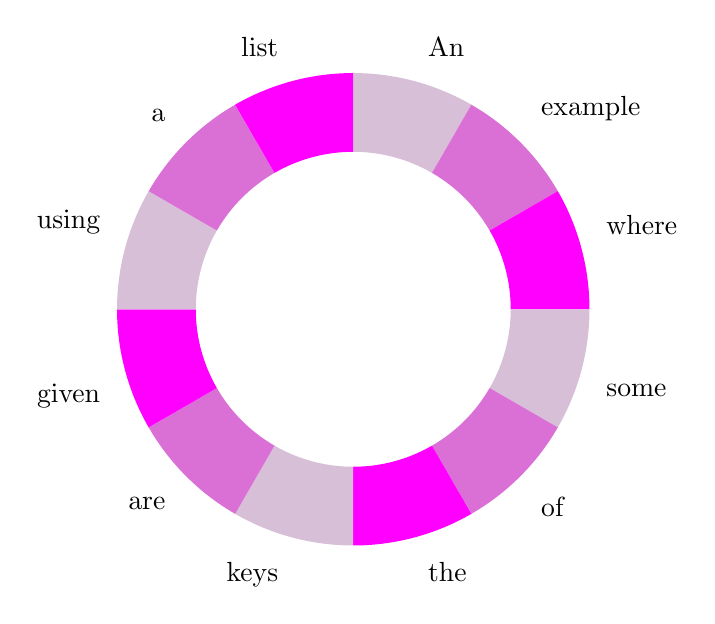
\begin{tikzpicture}
\wheelchart[
    data{list}={
        An,example,where,some,of,the,
        keys,are,given,using,a,list
    },
    slices style{list}={
        Thistle,Orchid,Fuchsia
    },
    total count=12
]{}
\end{tikzpicture}
\end{codeexample}
\begin{codeexample}[code only,preamble={\usepackage{listofitems}}]
\readlist\WCcolors{Thistle,Orchid,Fuchsia}

\setsepchar{ }
\readlist\WCdata{An example where some of the keys are given using a list}

data={\WCdata[\WCcount]},

slices style={
    /utils/exec={\pgfmathsetmacro{\WCcolornumber}{int(Mod({\WCcount-1},\WCcolorslen)+1)}},
    \WCcolors[\WCcolornumber]
},

total count=\WCdatalen,
\end{codeexample}
\begin{codeexample}[code only]
slices style{1,4,...,\WCdatalen}=Thistle,
slices style{2,5,...,\WCdatalen}=Orchid,
slices style{3,6,...,\WCdatalen}=Fuchsia,
\end{codeexample}
\item The following wheelchart can be obtained with the 3 possibilities below.
\begin{codeexample}[width=10cm]
\begin{tikzpicture}
\wheelchart[
    explode=\WCvarF,
    pie
]{\exampleforthismanual}
\end{tikzpicture}
\end{codeexample}
\begin{codeexample}[code only]
explode={\WCcount==3?0.5:(\WCcount==7?1:0)},
\end{codeexample}
\begin{codeexample}[code only]
explode{3}=0.5,
explode{7}=1,
\end{codeexample}
\end{itemize}
\begin{key}{/wheelchart/after slices=\marg{code} (initially \normalfont empty)}
The \meta{code} given to this key will be executed after each slice of the wheelchart.
\end{key}
\begin{key}{/wheelchart/anchor xsep=\marg{angle} (initially 5)}
\end{key}
\begin{key}{/wheelchart/anchor ysep=\marg{angle} (initially 5)}
These keys determine the default anchor of the key |data| in the case that |lines ext=0|. Note that rounding errors can occur in the computation of the angle which is used to determine the default anchor according to Table \ref{tableanchorofthekeydatainthecasethatlinesextequaltozero}.
\begin{table}[ht]
\centering
\begin{tabular}{ll}
 & Anchor of the key |data|\\
Angle (up to rounding errors) & in the case that |lines ext=0|\\\hline
$0$ & west\\
$90$ & south\\
$180$ & east\\
$270$ & north\\
For other angles not in $\{0,90,180,270\}$: & \\
$[0,\text{|anchor ysep|}]$ & west\\
$\ointerval{\text{|anchor ysep|}}{90-\text{|anchor xsep|}}$ & south west\\
$[90-\text{|anchor xsep|},90+\text{|anchor xsep|}]$ & south\\
$\ointerval{90+\text{|anchor xsep|}}{180-\text{|anchor ysep|}}$ & south east\\
$[180-\text{|anchor ysep|},180+\text{|anchor ysep|}]$ & east\\
$\ointerval{180+\text{|anchor ysep|}}{270-\text{|anchor xsep|}}$ & north east\\
$[270-\text{|anchor xsep|},270+\text{|anchor xsep|}]$ & north\\
$\ointerval{270+\text{|anchor xsep|}}{360-\text{|anchor ysep|}}$ & north west\\
$[360-\text{|anchor ysep|},360]$ & west\\
\end{tabular}
\caption{Anchor of the key \texttt{data} in the case that \texttt{lines ext=0}.}\label{tableanchorofthekeydatainthecasethatlinesextequaltozero}
\end{table}
\begin{codeexample}[width=10cm,preamble={\usepackage{siunitx}}]
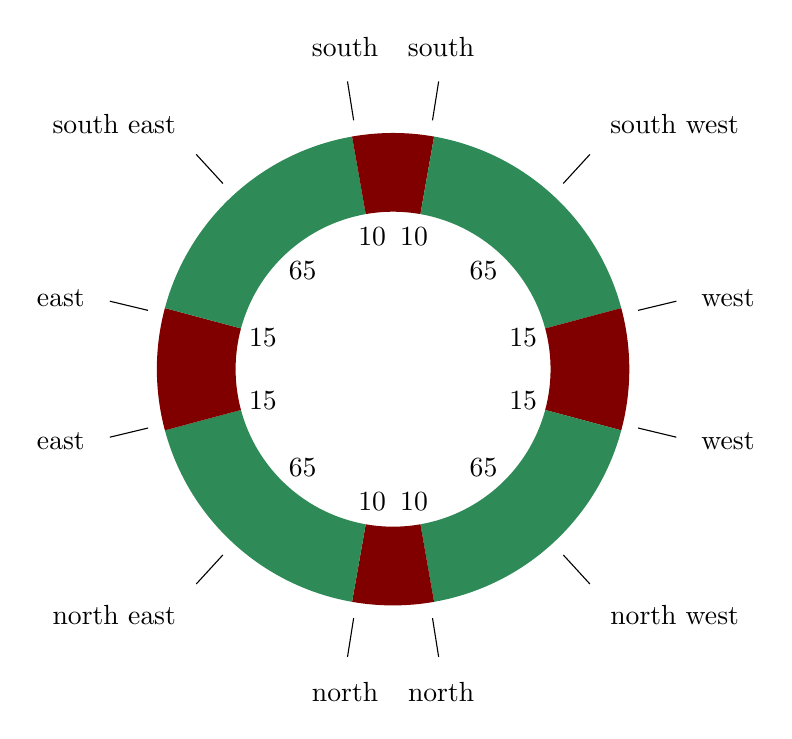
\begin{tikzpicture}
\wheelchart[
    anchor xsep=10,
    anchor ysep=15,
    data=\WCvarA,
    data angle pos=\WClistdap,
    inner data=\ang{\WClistvalue},
    inner data angle pos=\WClistdap,
    inner data sep=0.3,
    lines=0.5,
    lines angle pos=\WClistdap,
    slices style{list}={
        Maroon,SeaGreen,Maroon
    },
    value=\WClistvalue,
    WClistdap={0.9,0.5,0.1},
    WClistvalue={10,65,15,15,65,10}
]{%
    south,
    south west,
    west,
    west,
    north west,
    north,
    north,
    north east,
    east,
    east,
    south east,
    south%
}
\end{tikzpicture}
\end{codeexample}
The anchor of the key |data| can also be specified manually by using |data style={anchor=|\meta{anchor}|}|.
\end{key}
\begin{stylekey}{/wheelchart/arc=\marg{options} (initially \normalfont empty)}
If this key is set then an arc with the style determined by this key will be drawn following the plot for a slice of the wheelchart.
\end{stylekey}
\begin{key}{/wheelchart/arc around text=\opt{\meta{boolean}} (default true, initially false)}
If true then the arc with the style determined by the key |arc| will be split in two parts such that the gap between these two parts leaves space for the contents of the key |arc data|. The space between the arc and the contents of the key |arc data| can be increased with for example |~| in |arc data=~text~|.
\end{key}
\begin{key}{/wheelchart/arc data=\marg{text} (initially \normalfont empty)}
This key contains the \meta{text} which will be placed following the plot for a slice of the wheelchart using the decoration |text along path|. This requires the \tikzname{} library |decorations.text|. The style of this decoration is given as follows. First, the option |raise=-0.5ex| is given. Then |text align| is determined by the key |arc data align|. Thereafter, the style of the key |arc data style| is added.

Note that for example |\WCpercentage| follows the arc but |\WCperc| does not. Braces are required around some macros and for example |arc data={{{{\WCperc}}}}| requires 4 pairs of braces.
\end{key}
\begin{key}{/wheelchart/arc data align=\mchoice{center,left,right} (initially center)}
This key determines the alignment of the contents of the key |arc data|.
\end{key}
\begin{key}{/wheelchart/arc data angle pos=\marg{value} (initially 0.5)}
\end{key}
\begin{key}{/wheelchart/arc data angle shift=\marg{angle} (initially 0)}
These keys determine the position of the contents of the key |arc data| similar as the corresponding keys for the key |data|.
\end{key}
\begin{key}{/wheelchart/arc data dir=\marg{value} (initially 1)}
This key determines the direction of the contents of the key |arc data|. If the \meta{value} is positive then the direction is the same as the direction of the slice. If the \meta{value} is negative then the direction is reversed. The values |1| and |-1| are recommended. When the contents of the key |arc data| is placed, the corresponding domain for the plot is estimated. A warning is given when the contents of the key |arc data| did (possibly) not fit. In this case, the absolute value of the key |arc data dir| should be increased.
\end{key}
\begin{key}{/wheelchart/arc data pos=\marg{value} (initially 1)}
\end{key}
\begin{key}{/wheelchart/arc data sep=\marg{value} (initially 1ex/1cm)}
These keys determine the position of the contents of the key |arc data| similar as the corresponding keys for the key |data|.
\end{key}
\begin{stylekey}{/wheelchart/arc data style=\marg{options} (initially \normalfont empty)}
This key accepts a list of keys which will be applied to the decoration for the key |arc data|.
\end{stylekey}
\begin{stylekey}{/wheelchart/arc first half=\marg{options} (initially \normalfont empty)}
If |arc around text| is true then the arc with the style determined by the key |arc| will be split in two parts. The style determined by the key |arc first half| will be appended to the first half of the arc.
\end{stylekey}
\begin{key}{/wheelchart/arc pos=\marg{value} (initially 1)}
This key determines the position of the arc similar as the corresponding key for the key |data|.
\end{key}
\begin{stylekey}{/wheelchart/arc second half=\marg{options} (initially \normalfont empty)}
This key is similar to the key |arc first half| but will be appended to the second half of the arc.
\end{stylekey}
\begin{key}{/wheelchart/arc sep=\marg{value} (initially 1ex/1cm)}
This key determines the position of the arc similar as the corresponding key for the key |data|. Note that the actual distance is given by |0.5ex/1cm| plus |arc sep| to match the option |raise=-0.5ex| given to the decoration for the key |arc data|.
\begin{codeexample}[width=10cm,preamble={\usetikzlibrary{decorations.text}}]
\begin{tikzpicture}
\wheelchart[
    arc=\WCvarB,
    arc around text,
    arc data=~\WCvarC~,
    arc data dir={\WCmidangle<180?1:-1},
    arc data pos=1.2,
    arc data style={text color=\WCvarB},
    arc first half=dashed,
    arc pos=1.2,
    arc second half=->,
    data=,
    value=width("\WCvarC")
]{\exampleforthismanual}
\useasboundingbox (0,0)
    circle[radius=4];
\end{tikzpicture}
\end{codeexample}
\end{key}
\begin{key}{/wheelchart/at=\marg{point} (initially (0,0))}
This key defines the center of the wheelchart.
\end{key}
\begin{key}{/wheelchart/before slices=\marg{code} (initially \normalfont empty)}
The \meta{code} given to this key will be executed before each slice of the wheelchart.
\end{key}
\begin{key}{/wheelchart/caption=\marg{text} (initially \normalfont empty)}
This key contains the \meta{text} which will be placed below the wheelchart. The \meta{text} is placed in a node. The $x$ coordinate of this node is the $x$ coordinate of the center of the wheelchart, which is defined by the key |at|. In general, this is \emph{not} the same as the $x$ coordinate of the center of the |local bounding box| around the wheelchart. The $y$ coordinate of this node is at a value determined by the key |caption sep| below the south of the |local bounding box| around the wheelchart. The style of this node is given as follows. First, the options |anchor=north,align=center| are given. Thereafter, the style of the key |caption style| is added.
\end{key}
\begin{key}{/wheelchart/caption left=\marg{text} (initially \normalfont empty)}
This key contains the \meta{text} which will be placed below left of the wheelchart. The \meta{text} is placed in a node. This node is placed at a value determined by the key |caption left sep| below the south west of the |local bounding box| around the wheelchart. The style of this node is given as follows. First, the options |anchor=north west,align=left| are given. Thereafter, the style of the key |caption left style| is added.
\end{key}
\begin{key}{/wheelchart/caption left sep=\marg{value} (initially 0.5)}
The node where the contents of the key |caption left| is placed is at \meta{value} below the south west of the |local bounding box| around the wheelchart.
\end{key}
\begin{stylekey}{/wheelchart/caption left style=\marg{options} (initially \normalfont empty)}
This key accepts a list of keys which will be applied to the node where the contents of the key |caption left| is placed.
\end{stylekey}
\begin{key}{/wheelchart/caption sep=\marg{value} (initially 0.5)}
The $y$ coordinate of the node where the contents of the key |caption| is placed is at \meta{value} below the south of the |local bounding box| around the wheelchart.
\end{key}
\begin{stylekey}{/wheelchart/caption style=\marg{options} (initially \normalfont empty)}
This key accepts a list of keys which will be applied to the node where the contents of the key |caption| is placed.
\begin{codeexample}[width=10cm]
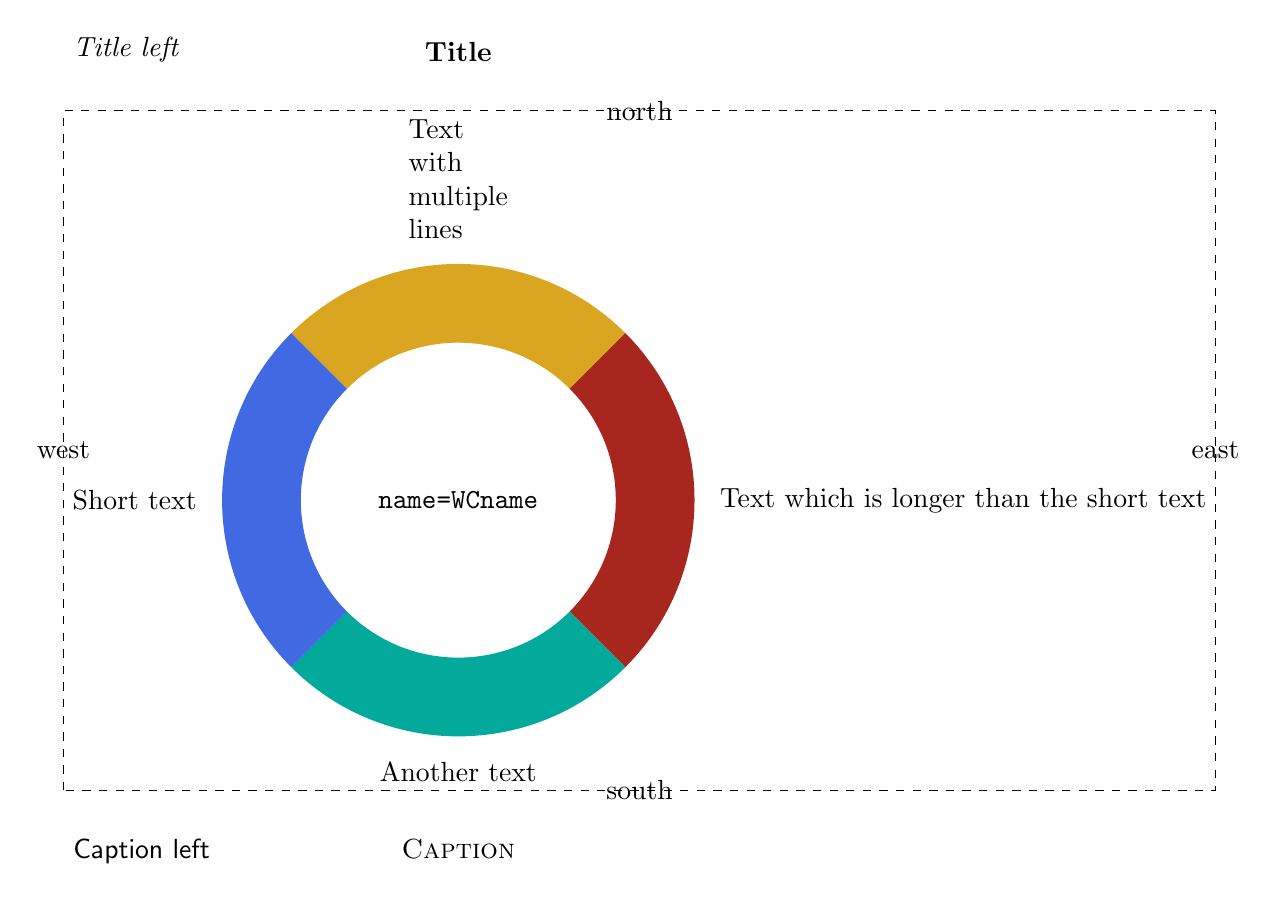
\begin{tikzpicture}
\wheelchart[
    at={(5,2)},
    caption=Caption,
    caption style={font=\scshape},
    caption left=Caption left,
    caption left style={font=\sffamily},
    middle=\texttt{name=WCname},
    name=WCname,
    start half,
    title=Title,
    title style={font=\bfseries},
    title left=Title left,
    title left style={font=\em}
]{%
    1/Goldenrod/Text\\with\\multiple\\lines,
    1/Mahogany/Text which is longer than the short text,
    1/JungleGreen/Another text,
    1/RoyalBlue/Short text%
}
\draw[dashed] (WCname.south west) rectangle (WCname.north east);
\foreach\pos in {north,east,south,west}{
    \node at (WCname.\pos) {\pos};
}
\end{tikzpicture}
\end{codeexample}
\end{stylekey}
\begin{stylekey}{/wheelchart/contour=\marg{options} (initially \normalfont empty)}
If this key is set then a contour with the style determined by this key will be drawn around the wheelchart. This key does \emph{not} apply if a plot is used.
\end{stylekey}
\begin{key}{/wheelchart/counterclockwise=\opt{\meta{boolean}} (default true, initially false)}
If true, the wheelchart will be drawn counterclockwise instead of clockwise.
\end{key}
\begin{key}{/wheelchart/data=\marg{text} (initially \textbackslash WCvarC)}
This key contains the \meta{text} which will be placed at each slice of the wheelchart. This can be suppressed by using |data={}|. The \meta{text} is placed in a node. The style of this node is given as follows. First, the anchor is set following Table \ref{tableanchorofthekeydatainthecasethatlinesextequaltozero} and Table \ref{tableanchorofthekeydatainthecasethatlinesextdifferentfromzero}. Then the option |align=left| is added. Thereafter, the style of the key |data style| is added.
\end{key}
\begin{key}{/wheelchart/data angle pos=\marg{value} (initially 0.5)}
\end{key}
\begin{key}{/wheelchart/data angle shift=\marg{angle} (initially 0)}
\end{key}
\begin{key}{/wheelchart/data pos=\marg{value} (initially 1)}
\end{key}
\begin{key}{/wheelchart/data sep=\marg{value} (initially 0.2)}
The position of the contents of the key |data| is determined as follows.
\begin{enumerate}
\item The inner plot is evaluated in the point with as angle the convex combination with as parameter the key |data angle pos| of the inner start angle and the inner end angle, added with the key |data angle shift| in degrees (taking into account the key |counterclockwise|) and as radius the inner radius minus the key |data sep|.
\item The outer plot is evaluated in the similar point but using the outer start angle, the outer end angle and the outer radius plus the key |data sep|.
\item If $\text{|lines|}\neq 0$ then the values of the keys |lines sep| and |lines| are added to the radii above, in addition to the key |data sep|.
\item The contents of the key |data| is placed at the convex combination with as parameter the key |data pos| of the previous two points.
\end{enumerate}
\begin{codeexample}[]
\begin{tikzpicture}
\wheelchart[
    data angle pos{2}=0.3,
    data angle pos{6}=0.8,
    data angle shift{3}=-0.1,
    data angle shift{5}=0.1,
    data pos=\WClistB,
    data sep=0,
    lines{1,2,4,6,7}=0.5,
    lines{3,5}=1,
    lines angle pos{1}=0.8,
    lines angle shift{7}=-0.2,
    lines ext=\WClistA,
    lines ext dir{1,...,3}=left,
    lines ext dir{4,...,7}=right,
    lines ext fixed,
    lines ext fixed left=-1,
    lines ext fixed right=7,
    lines pos=\WClistB,
    lines sep=0.2*\WClistA,
    xbar={6}{1.5},
    WClistA={1,0},
    WClistB={0,1},
    wheel data=\WCperc,
    wheel data pos=0.5,
    wheel data pos{1}=1,
    wheel data pos{4}=0,
    wheel data sep=0.2
]{\exampleforthismanual}
\end{tikzpicture}
\end{codeexample}
\end{key}
\begin{stylekey}{/wheelchart/data style=\marg{options} (initially \normalfont empty)}
This key accepts a list of keys which will be applied to the node where the contents of the key |data| is placed.
\end{stylekey}
\begin{key}{/wheelchart/discrete=\opt{\meta{boolean}} (default true, initially false)}
If true then \tikzname{} pics are placed with the \meta{code} determined by the key |discrete pic|. The number of pics is determined by the key |value|. It is required to set the key |discrete space at borders|.
\end{key}
\begin{key}{/wheelchart/discrete factor=\marg{value} (initially 1)}
The algorithm to place the \tikzname{} pics depends on the \meta{value}. The value |1| is recommended.
\end{key}
\begin{key}{/wheelchart/discrete partitioning=\mchoice{angle,radius} (initially radius)}
\begin{description}
\item[\texttt{angle}] In this case, the \tikzname{} pics are placed uniformly with respect to the angle.
\item[\texttt{radius}] In this case, the \tikzname{} pics are placed uniformly with respect to the radius.
\end{description}
These options are illustrated in the examples below.
\begin{codeexample}[]
\begin{tikzpicture}
\pgfkeys{
    /wheelchart,
    data=,
    discrete,
    discrete pic={\fill (0,0) circle[radius=3pt];},
    discrete space at borders=false,
    middle style={font=\ttfamily},
    start angle=180,
    total angle=180,
    value=\WCvarA/2
}
\foreach\angle in {0,...,27}{
    \draw ({180*(\angle/27)}:2)--({180*(\angle/27)}:3);
}
\wheelchart[
    discrete partitioning=angle,
    middle={discrete\\partitioning=angle}
]{\exampleforthismanual}
\foreach\radius in {0,...,3}{
    \draw ({9+\radius/3},0) arc[start angle=0,end angle=180,radius={2+\radius/3}];
}
\wheelchart[
    at={(7,0)},
    middle={discrete\\partitioning=radius}
]{\exampleforthismanual}
\end{tikzpicture}
\end{codeexample}
\end{key}
\begin{key}{/wheelchart/discrete pic=\marg{code} (initially \normalfont empty)}
The \meta{code} determines the \tikzname{} pics.
\begin{codeexample}[width=10cm]
\begin{tikzpicture}[yscale=-1]
\wheelchart[
    data=,
    discrete,
    discrete pic={
        \fill[draw=black] (-0.3,-0.3)
            rectangle +(0.6,0.6);
        \node[black] at (0,0)
            {\WCcountdiscrete};
    },
    discrete space at borders,
    value=\WCvarA/2,
    ybar={8}{8}
]{\exampleforthismanual}
\end{tikzpicture}
\end{codeexample}
\end{key}
\begin{key}{/wheelchart/discrete sort=\mchoice{angle,radius} (initially angle)}
\begin{description}
\item[\texttt{angle}] In this case, the \tikzname{} pics are ordered with respect to the angle.
\item[\texttt{radius}] In this case, the \tikzname{} pics are ordered with respect to the radius.
\end{description}
These options are illustrated in the examples below.
\begin{codeexample}[]
\begin{tikzpicture}
\pgfkeys{
    /wheelchart,
    data=,
    discrete,
    discrete pic={\shade[ball color=\WCvarB] (0,0) circle[radius=4pt];},
    discrete space at borders=false,
    middle style={font=\ttfamily},
    start angle=180,
    total angle=180,
    value=\WCvarA/2
}
\wheelchart[
    legend columns=4,
    legend row={\tikz\shade[ball color=\WCvarB] (0,0) circle[radius=4pt]; & \WCvarC & \WCperc},
    legend={\node[anchor=north] at (3.5,-1) {\begin{tabular}{*{4}{l@{ }lr}}\WClegend\end{tabular}};},
    middle={discrete sort=angle}
]{\exampleforthismanual}
\wheelchart[
    at={(7,0)},
    discrete sort=radius,
    middle={discrete sort=radius}
]{\exampleforthismanual}
\end{tikzpicture}
\end{codeexample}
\end{key}
\begin{key}{/wheelchart/discrete space at borders=\opt{\meta{boolean}} (default true)}
This key determines whether space is left at the begin and end where the \tikzname{} pics are placed. For example, suppose that $3$ \tikzname{} pics are placed at positions between $0$ and $1$. If |discrete space at borders| is true then these are placed at the positions $\frac{1}{6}$, $\frac{3}{6}$ and $\frac{5}{6}$. If |discrete space at borders| is false then these are placed at the positions $0$, $\frac{1}{2}$ and $1$.

This key deliberately has no initial value in order to force awareness of the consequences of the settings of this key. In the example below, the cyan \tikzname{} pics are aligned if |discrete space at borders| is false while this is \emph{not} the case if |discrete space at borders| is true.
\begin{codeexample}[]
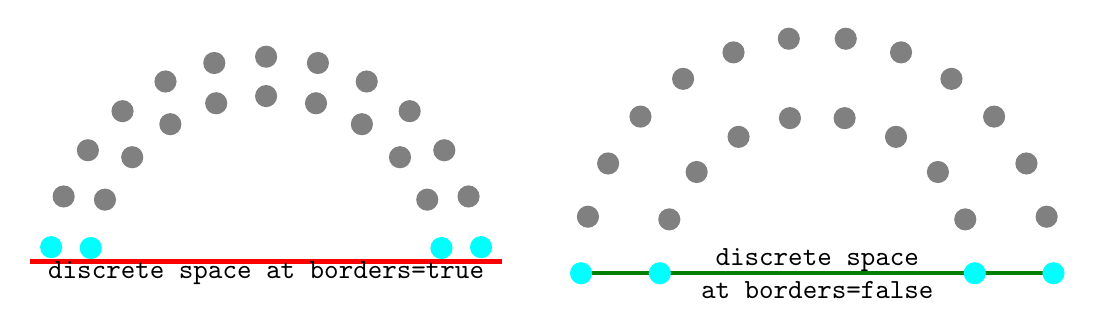
\begin{tikzpicture}
\pgfkeys{
    /wheelchart,
    discrete,
    discrete pic={\fill (0,0) circle[radius=4pt];},
    middle style={font=\ttfamily},
    start angle=180,
    total angle=180
}
\draw[Red,ultra thick] (-3,0.15)--+(6,0);
\wheelchart[
    discrete space at borders,
    middle={discrete space at borders=true}
]{2/Cyan/,20/Gray/,2/Cyan/}
\draw[Green,ultra thick] (4,0)--+(6,0);
\wheelchart[
    at={(7,0)},
    discrete space at borders=false,
    middle={discrete space\\at borders=false}
]{2/Cyan/,20/Gray/,2/Cyan/}
\end{tikzpicture}
\end{codeexample}
In the example below, the red and green \tikzname{} pics overlap if |discrete space at borders| is false while this is \emph{not} the case if |discrete space at borders| is true.
\begin{codeexample}[]
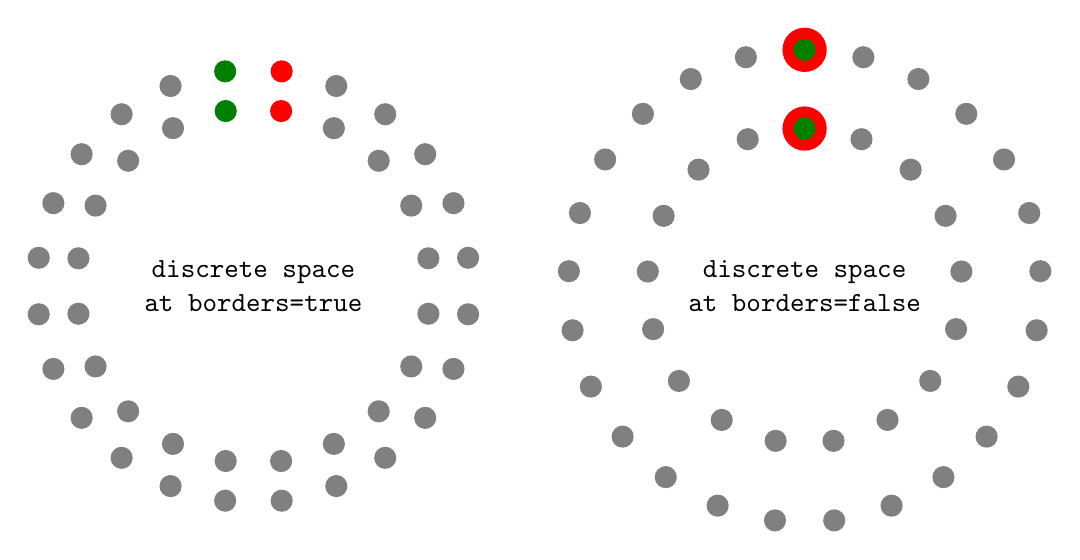
\begin{tikzpicture}
\pgfkeys{
    /wheelchart,
    discrete,
    discrete pic={\fill (0,0) circle[radius=\WClistradius pt];},
    middle style={font=\ttfamily}
}
\wheelchart[
    discrete space at borders,
    middle={discrete space\\at borders=true},
    WClistradius=4
]{2/Red/,40/Gray/,2/Green/}
\wheelchart[
    at={(7,0)},
    discrete space at borders=false,
    middle={discrete space\\at borders=false},
    WClistradius={8,4,4}
]{2/Red/,40/Gray/,2/Green/}
\end{tikzpicture}
\end{codeexample}
\end{key}
\begin{key}{/wheelchart/domain=\marg{start}:\marg{end}}
This key sets |counterclockwise|, |start angle| to \meta{start} and |total angle| to $\text{\meta{end}}-\text{\meta{start}}$.
\end{key}
\begin{key}{/wheelchart/etoc code=\marg{code} (initially \textbackslash tableofcontents)}
The \meta{code} will be executed to build the \meta{wheelchart data} if the key |etoc level| is used.
\end{key}
\begin{key}{/wheelchart/etoc count total pages=\marg{number} (initially 0)}
If the key |etoc level| is used then the number of pages of the last section depends on \meta{number} which can for example represent the total number of pages in the document or the number of pages before the start of the Appendix or the Index. For example, |etoc count total pages=\totalpages| can be used. To provide the command |\totalpages|, this requires |\usepackage[page]{totalcount}|, which should normally be loaded \emph{before} the package |wheelchart| to give a correct result.
\end{key}
\begin{key}{/wheelchart/etoc level=\marg{level}}
If this key is used then the \meta{wheelchart data} of the command |\wheelchart| can be left empty and is defined to match the sections of the level defined by \meta{level}. Here, |\WCetocthelinkedname| corresponds to |\etocthelinkedname|, |\WCetocthelinkednumber| to |\etocthelinkednumber|, |\WCetocthelinkedpage| to |\etocthelinkedpage|, |\WCetocthename| to |\etocthename|, |\WCetocthenumber| to |\etocthenumber| and |\WCetocthepage| to |\etocthepage|. The package |etoc| is required to provide these commands. Furthermore, |\WCetocthenumberofpages| corresponds to the number of pages of the current section. For the last section, this depends on the value of the key |etoc count total pages|.
\end{key}
\begin{key}{/wheelchart/etoc name=\marg{name} (initially \normalfont empty)}
The resulting \meta{wheelchart data} from the key |etoc level| is stored globally and can be reused later with the key |etoc use name|.
\end{key}
\begin{key}{/wheelchart/etoc use name=\marg{name}}
If this key is used then the \meta{wheelchart data} is reused from where |etoc name| has the same \meta{name}.
\end{key}
\begin{key}{/wheelchart/expand list=\mchoice{false,once,true} (initially once)}
\begin{description}
\item[\texttt{false}] In this case, the \meta{wheelchart data} of the command |\wheelchart| will not be expanded.
\item[\texttt{once}] In this case, the \meta{wheelchart data} of the command |\wheelchart| will be expanded once.
\item[\texttt{true}] In this case, the \meta{wheelchart data} of the command |\wheelchart| will be fully expanded.
\end{description}
The following example illustrates the difference between the possible values of the key |expand list|.
\begin{codeexample}[width=10cm]
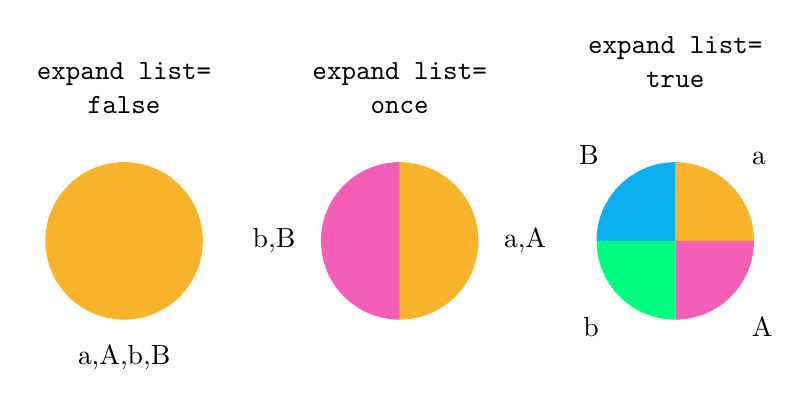
\begin{tikzpicture}
\def\WClistA{a,A}
\def\WClistB{b,B}
\def\WCdata{\WClistA,\WClistB}
\foreach\expandlist [count=\n] in
    {false,once,true}{
\wheelchart[
    at={({3.5*\n},0)},
    data=\WCvarA,
    expand list=\expandlist,
    radius={0}{1},
    slices style{list}={
        Dandelion,CarnationPink,
        SpringGreen,ProcessBlue
    },
    title={expand list=\\\expandlist},
    title style={font=\ttfamily},
    value=1
]{\WCdata}
}
\end{tikzpicture}
\end{codeexample}
The initial setting |expand list=once| works in most situations, even when commands such as |\ref|, |\cite| and |\textbf| are used such as in the example below.
\begin{codeexample}[width=10cm]
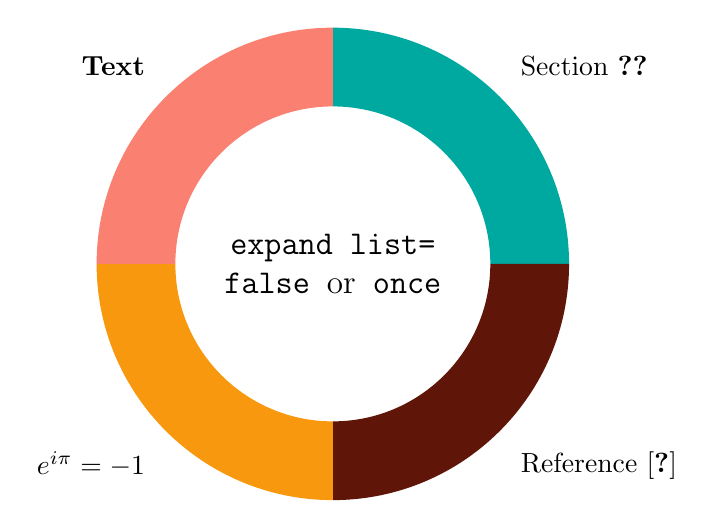
\begin{tikzpicture}
\wheelchart[
    %expand list=false,%false also works
    %expand list=true,%true doesn't work
    middle={expand list=\\false %
        {\normalfont or} once},
    middle style={font=\large\ttfamily}
]{%
    1/Emerald/Section \ref{Keys},
    1/Sepia/Reference \cite{TtTaPGFp},
    1/YellowOrange/{$e^{i\pi}=-1$},
    1/Salmon/\textbf{Text}%
}
\end{tikzpicture}
\end{codeexample}
In the following example, the \meta{wheelchart data} from the previous example is stored in a macro. In this case, we have to use the initial setting |expand list=once|.
\begin{codeexample}[width=10cm]
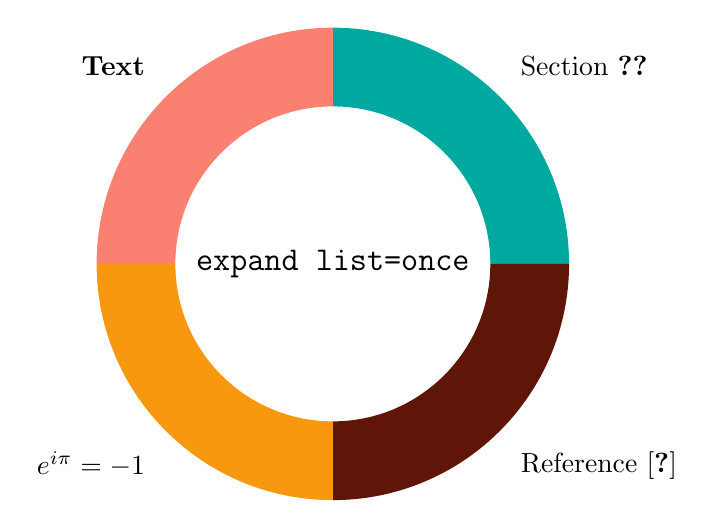
\begin{tikzpicture}
\def\WClist{%
    1/Emerald/Section \ref{Keys},
    1/Sepia/Reference \cite{TtTaPGFp},
    1/YellowOrange/{$e^{i\pi}=-1$},
    1/Salmon/\textbf{Text}%
}
\wheelchart[
    %expand list=false,
    %expand list=true,
    %false and true do not work
    middle={expand list=once},
    middle style={font=\large\ttfamily}
]{\WClist}
\end{tikzpicture}
\end{codeexample}
In the example below, we have to use |expand list=true|.
\begin{codeexample}[width=10cm]
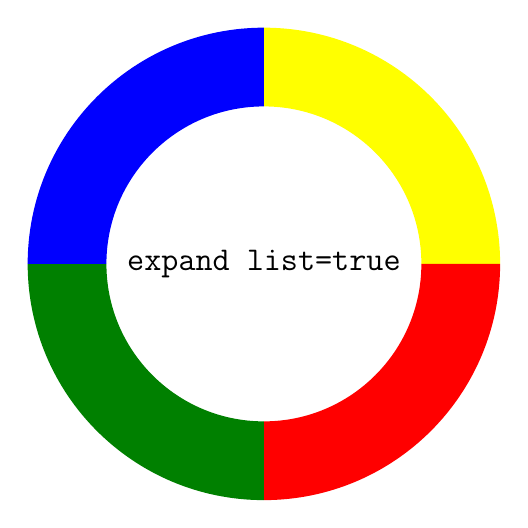
\begin{tikzpicture}
\def\WCcolorsA{Yellow,Red}
\def\WCcolorsB{Green,Blue}
\wheelchart[
    data=,
    expand list=true,%false and once
                     %do not work
    middle={expand list=true},
    middle style={font=\large\ttfamily},
    slices style=\WCvarA,
    value=1
]{\WCcolorsA,\WCcolorsB}
\end{tikzpicture}
\end{codeexample}
In the example below, we have to use |expand list=true| and the command |\expandonce| from the package |etoolbox|.
\begin{codeexample}[width=10cm,preamble={\usepackage{etoolbox}}]
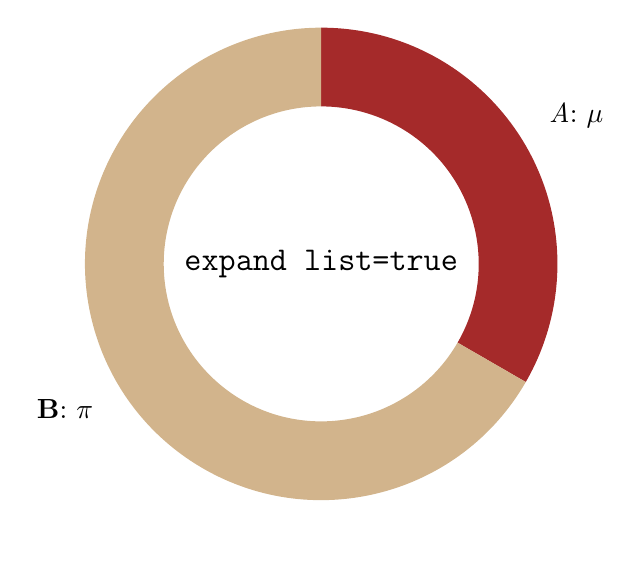
\begin{tikzpicture}
\def\WCsliceA{1/Brown/{\emph{A}: $\mu$}}
\def\WCsliceAfinal{\expandonce\WCsliceA}
\def\WCsliceB{2/Tan/{\textbf{B}: $\pi$}}
\def\WCsliceBfinal{\expandonce\WCsliceB}
\wheelchart[
    expand list=true,%false and once
                     %do not work
    middle={expand list=true},
    middle style={font=\large\ttfamily}
]{\WCsliceAfinal,\WCsliceBfinal}
%\WCsliceA and \WCsliceB do not work
\end{tikzpicture}
\end{codeexample}
\end{key}
\begin{key}{/wheelchart/expand list items=\mchoice{false,once,true} (initially false)}
This key is similar to the key |expand list| but applies to the items in the \meta{wheelchart data} of the command |\wheelchart| which correspond to a slice of the wheelchart.
\begin{codeexample}[width=10cm]
\def\WClistA{a/b}%
\def\WClistB{c/d}%
\def\WCdata{\WClistA/\WClistB}%
\texttt{expand list items}%
\foreach\expandlistitems in
    {false,once,true}{%
\wheelchart[
    expand list=false,
    expand list items=\expandlistitems,
    legend={; \texttt{\expandlistitems}:
        \WCvarA},
    legend only,
    value=1
]{\WCdata}%
}
\end{codeexample}
\end{key}
\begin{key}{/wheelchart/explode=\marg{value} (default 0.2, initially 0)}
This key will shift the slices of the wheelchart with \meta{value} with respect to the center of the wheelchart.
\end{key}
\begin{key}{/wheelchart/for loop end=\marg{code} (initially \normalfont empty)}
The slices of the wheelchart, the wheel lines determined by the key |wheel lines| and the different kinds of data are placed in for loops. If the key |for loop end| is set then the \meta{code} given to this key will be executed at the end of the body of these for loops.
\end{key}
\begin{key}{/wheelchart/for loop start=\marg{code} (initially \normalfont empty)}
This key is similar to the key |for loop end| but the \meta{code} given to this key will be executed at the start of the body of the for loops.
\end{key}
\begin{key}{/wheelchart/gap=\marg{value} (default 0.05, initially 0)}
The \meta{value} of this key defines half the distance between two slices of the wheelchart. This key does \emph{not} apply if a plot is used.
\end{key}
\begin{key}{/wheelchart/gap max angle=\marg{angle} (initially 180)}
If the value of the key |gap| is too large then a slice can partly disappear such as for example below when |gap max angle| is \ang{155}. The \meta{angle} of the key |gap max angle| determines the inner arc of the slice as illustrated in the examples below.
\begin{codeexample}[preamble={\usepackage{siunitx}}]
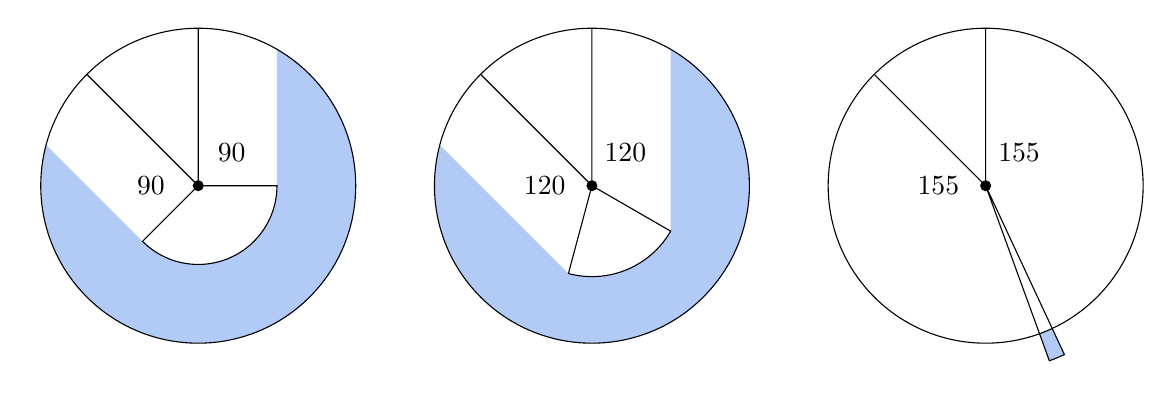
\begin{tikzpicture}
\foreach\gapmaxangle [count=\n] in {90,120,155}{
\begin{scope}[shift={({5*\n},0)}]
\wheelchart[
    gap=1,
    gap max angle=\gapmaxangle,
    radius={0}{2},
    total angle=315
]{1/CornflowerBlue!50/}
\fill (0,0) circle[radius=2pt];
\draw (0,0) circle[radius=2];
\draw (135:2)--(0:0)--(90:2);
\draw (0:0)--({135+\gapmaxangle}:{1/sin(\gapmaxangle)}) arc[start angle={135+\gapmaxangle},
    end angle={450-\gapmaxangle},radius={1/sin(\gapmaxangle)}]--cycle;
\node at (45:0.6) {\ang{\gapmaxangle}};
\node at (180:0.6) {\ang{\gapmaxangle}};
\end{scope}
}
\end{tikzpicture}
\end{codeexample}
\end{key}
\begin{key}{/wheelchart/gap polar=\marg{value} (default 1, initially 0)}
The \meta{value} of this key defines half the polar gap in degrees between two slices of the wheelchart.

Note the difference between the keys |explode|, |gap| and |gap polar|. This is illustrated in the examples below.
\begin{codeexample}[width=10cm]
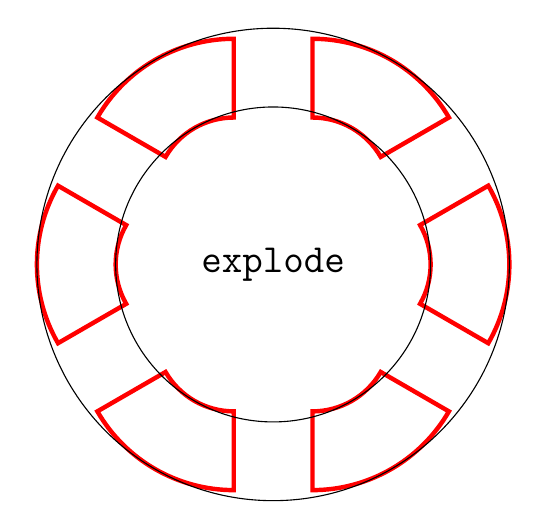
\begin{tikzpicture}
\wheelchart[
    explode=1,
    middle={\Large\texttt{explode}},
    radius={1}{2},
    slices style={
        draw=Red,
        fill=none,
        ultra thick
    },
    total count=6
]{}
\draw (0,0) circle[radius=2];
\draw (0,0) circle[radius=3];
\end{tikzpicture}
\end{codeexample}
\begin{codeexample}[width=10cm]
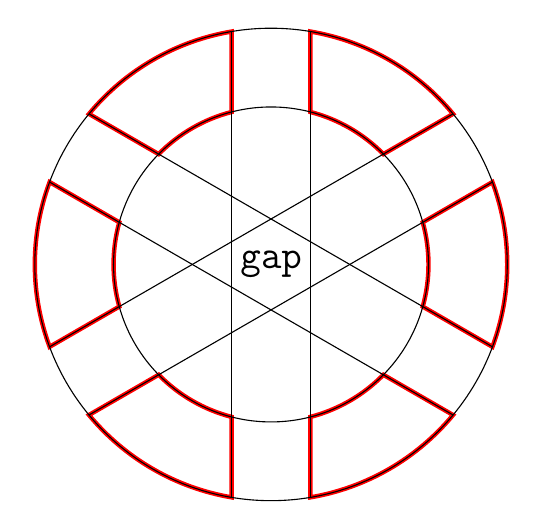
\begin{tikzpicture}
\wheelchart[
    gap=0.5,
    middle={\Large\texttt{gap}},
    slices style={
        draw=Red,
        fill=none,
        ultra thick
    },
    total count=6
]{}
\draw (0,0) circle[radius=2];
\draw (0,0) circle[radius=3];
\foreach\a in {0,60,120}{
\foreach\x in {-0.5,0.5}{
\draw[rotate=\a] (\x,{sqrt(3^2-0.5^2)})
    --(\x,{-sqrt(3^2-0.5^2)});
}
}
\end{tikzpicture}
\end{codeexample}
\begin{codeexample}[width=10cm]
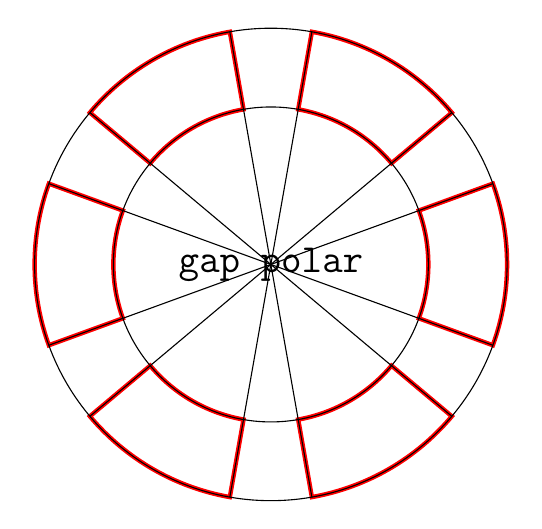
\begin{tikzpicture}
\wheelchart[
    gap polar=10,
    middle={\Large\texttt{gap polar}},
    slices style={
        draw=Red,
        fill=none,
        ultra thick
    },
    total count=6
]{}
\draw (0,0) circle[radius=2];
\draw (0,0) circle[radius=3];
\foreach\a in {30,90,150}{
\foreach\t in {-10,10}{
\draw ({\t+\a}:3)--({\t+\a+180}:3);
}
}
\end{tikzpicture}
\end{codeexample}
\end{key}
\begin{key}{/wheelchart/gap radius=\marg{value} (default 0.05, initially 0)}
The \meta{value} of this key will be added to |inner radius| and substracted from |outer radius|.
\begin{codeexample}[width=10cm,preamble={\usepackage{siunitx}}]
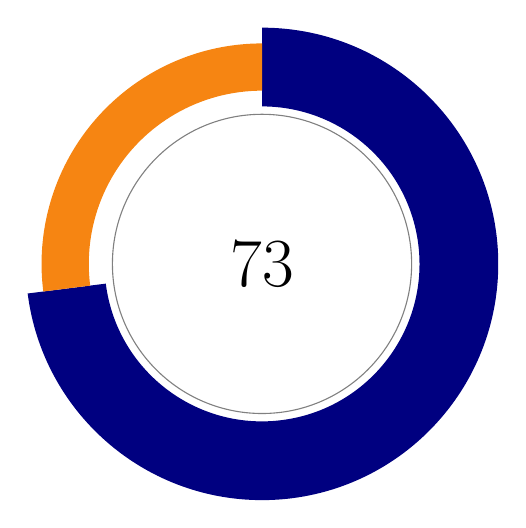
\begin{tikzpicture}
\def\n{73}
\wheelchart[
    data=,
    gap radius=\WCvarC,
    middle={\Huge\qty{\n}{\percent}}
]{%
    \n/NavyBlue/0,
    {100-\n}/BurntOrange/0.2%
}
\draw[Gray] (0,0) circle[radius=1.9];
\end{tikzpicture}
\end{codeexample}
\end{key}
\begin{key}{/wheelchart/header=\marg{list}}
The items in the \meta{list} determine the names in the macros |\|\meta{prefix}\meta{name}.
\end{key}
\begin{key}{/wheelchart/header prefix=\marg{prefix} (initially WC)}
The \meta{prefix} is used in the macros |\|\meta{prefix}\meta{name}.
\end{key}
\begin{key}{/wheelchart/inner data=\marg{text} (initially \normalfont empty)}
This key contains the \meta{text} which will be placed at each slice of the wheelchart. The \meta{text} is placed in a node. The style of this node is given as follows. First, the option |align=left| is given. Thereafter, the style of the key |inner data style| is added.
\end{key}
\begin{key}{/wheelchart/inner data angle pos=\marg{value} (initially 0.5)}
\end{key}
\begin{key}{/wheelchart/inner data angle shift=\marg{angle} (initially 0)}
\end{key}
\begin{key}{/wheelchart/inner data pos=\marg{value} (initially 0)}
\end{key}
\begin{key}{/wheelchart/inner data sep=\marg{value} (initially 0.2)}
These keys determine the position of the contents of the key |inner data| similar as the corresponding keys for the key |data|. No lines are drawn for the inner data.
\end{key}
\begin{stylekey}{/wheelchart/inner data style=\marg{options} (initially \normalfont empty)}
This key accepts a list of keys which will be applied to the node where the contents of the key |inner data| is placed.
\end{stylekey}
\begin{key}{/wheelchart/inner plot=\marg{code}}
The \meta{code} is a coordinate definition which will be used for the inner parts of the slices of the wheelchart. In the \meta{code}, |#1| and |#2| can be used where |#1| corresponds to the angle and |#2| corresponds to the radius. For example, a circle can be obtained with |inner plot={{#1}:{#2}}|.
\end{key}
\begin{stylekey}{/wheelchart/inner plot style=\marg{options} (initially \normalfont empty)}
This key accepts a list of keys which will be applied to the plot determined by the key |inner plot|.
\end{stylekey}
\begin{key}{/wheelchart/inner radius=\marg{value} (initially 2)}
The \meta{value} of this key defines the inner radius of the wheelchart.
\end{key}
\begin{key}{/wheelchart/legend=\marg{code} (initially \normalfont empty)}
The \meta{code} given to this key will be executed at the end of the command |\wheelchart|.
\end{key}
\begin{key}{/wheelchart/legend columns=\marg{number} (initially 1)}
If the key |legend row| is used then the maximum number of times that the \meta{code} given to the key |legend row| appears on one row is determined by \meta{number}. The environment (for example |tabular|, |tabularx| from the package |tabularx|, |tabulary| from the package |tabulary| or |tblr| from the package |tabularray|) which contains the macro |\WClegend| needs to have a suitable column specification according with \meta{number} and the key |legend row|.
\end{key}
\begin{key}{/wheelchart/legend entry=\marg{code} (initially \normalfont empty)}
The \meta{code} given to this key will be executed for each slice of the wheelchart.
\end{key}
\begin{key}{/wheelchart/legend only=\opt{\meta{boolean}} (default true, initially false)}
If true then only the legend is constructed. This does \emph{not} apply to the key |legend entry|.

In this case it is \emph{not} necessary to place the command |\wheelchart| in a |tikzpicture| environment.
\begin{codeexample}[width=10cm,preamble={\usepackage{tikzlings}}]
\wheelchart[
    header={animal,accessory},
    legend columns=3,
    legend only,
    legend row={\tikz[scale=0.3]{
        \csname \WCanimal\endcsname[
            signpost=\WCcount,
            \WCaccessory
        ]} & \WCanimal},
    legend={%
        \begin{tabular}{*{3}{cl}}
        \multicolumn{6}{c}{%
            \WCtotalcount{} animals%
            from the package%
            \texttt{tikzlings}}\\\hline
        \WClegend\hline
        \end{tabular}%
    },
    separator columns={{ }},
    separator rows=;,
    value=1
]{%
    bear basket;
    bee book;
    bug chef;
    cat crown;
    elephant football;
    koala handbag;
    owl hat;
    panda icecream;
    penguin milkshake;
    snowman santa;
    squirrel shovel%
}
\end{codeexample}
\end{key}
\begin{key}{/wheelchart/legend row=\marg{code}}
If this key is set then a legend consisting of rows for an environment such as |tabular|, |tabularx| from the package |tabularx|, |tabulary| from the package |tabulary| or |tblr| from the package |tabularray| is constructed using the \meta{code} for each slice of the wheelchart.

If a |tblr| environment from the package |tabularray| is used then the option |expand=\WClegend| needs to be given to this |tblr| environment and |\UseTblrLibrary{counter}| is required.

The maximum number of times that the \meta{code} appears on one row is determined by the key |legend columns|.

The code automatically inserts |&| and |\\| after the \meta{code} if necessary.

The result is stored in the macro |\WClegend|.
\begin{codeexample}[preamble={\usepackage{tabularray}
\UseTblrLibrary{counter,siunitx}}]
\begin{tikzpicture}
\wheelchart[
    after slices={
        \pgfdeclareradialshading{WCshading}{\pgfpoint{0cm}{0cm}}{
            color(0bp)=(\WCvarB);
            color(16.66666bp)=(\WCvarB);%2/3 * 25bp
            color(20.83333bp)=(\WCvarB!10);%2.5/3 * 25bp
            color(25bp)=(\WCvarB);
            color(50bp)=(\WCvarB)
        }
        \shade[even odd rule,shading=WCshading] (0,0) circle[radius=3] circle[radius=2];
    },
    data=,
    legend row={\tikz\fill[\WCvarB] (0,0) rectangle (0.3,0.3);%
         & \WCvarC & \WCvarA & \WCpercentagerounded & \WCvarD},
    legend={
        \node[anchor=west] at (3.5,0) {%
            \begin{tblr}[expand=\WClegend]{
                colspec={llS[table-format=3.0]S[table-format=2.0{\,\unit{\percent}}]l},
                column{1}={rightsep=0pt,appto={\ }},
                column{2}={leftsep=0pt},
                cell{2-Y}{4}={appto={\,\unit{\percent}}},
                row{1}={guard}
            }
             & Fruit & Value & Percentage & Vitamins\\\hline
            \WClegend\hline
             & \textbf{Total} & \WCtotalnum & & \\
            \end{tblr}%
        };
    },
    slices style={
        fill=none,
        clip
    }
]{\exampleforthismanual}
\end{tikzpicture}
\end{codeexample}
\end{key}
\begin{key}{/wheelchart/lines=\marg{value} (default 1, initially 0)}
The \meta{value} is used in the positioning of the contents of the key |data|. The end point of the lines is determined similarly but without the key |data sep|.
\begin{codeexample}[width=10cm,preamble={\usepackage{siunitx}}]
\begin{tikzpicture}
\def\WCtest#1#2{%
    \pgfmathparse{
        \WCpercentage>10?"#1":"#2"
    }%
    \pgfmathresult%
}
\wheelchart[
    data=\WCtest{}{\WCperc},
    lines={\WCpercentage>10?0:0.5},
    lines style={dotted,thick},
    pie,
    slices style={
        bottom color=\WCvarB,
        top color=\WCvarB!80!black,
        shading angle=\WCmidangle-90
    },
    wheel data=\WCtest{\WCperc}{}
]{\exampleforthismanual}
\end{tikzpicture}
\end{codeexample}
\end{key}
\begin{key}{/wheelchart/lines angle pos=\marg{value} (initially 0.5)}
\end{key}
\begin{key}{/wheelchart/lines angle shift=\marg{angle} (initially 0)}
These keys are similar to the corresponding keys for |data| but determine the start point of the lines.
\end{key}
\begin{key}{/wheelchart/lines ext=\marg{value} (default 0.5, initially 0)}
If the \meta{value} of this key is nonzero and |lines ext fixed| is false then the lines between the wheelchart and the contents of the key |data| will be extended horizontally with a length defined by \meta{value}.
\end{key}
\begin{key}{/wheelchart/lines ext bottom dir=\mchoice{left,right} (initially right)}
\end{key}
\begin{key}{/wheelchart/lines ext dir=\mchoice{left,right}}
The default direction in which the lines between the wheelchart and the contents of the key |data| will be extended horizontally if $\text{|lines ext|}\neq 0$ is determined by Table \ref{tablelinesextdir} and illustrated in the following example. This can be overruled by giving an explicit value to this key. Note that rounding errors can occur in the computation of the angle which is used to determine the default direction according to Table \ref{tablelinesextdir}.
\begin{table}[ht]
\centering
\begin{tabular}{ll}
 & The direction in which the lines between the\\
 & wheelchart and the contents of the key |data| will\\
 & be extended horizontally if $\text{|lines ext|}\neq 0$ and\\
Angle (up to rounding errors) & if the key |lines ext dir| is not used\\\hline
$\rinterval{0}{90-\text{|lines ext dirsep|}}$ & right\\
$[90-\text{|lines ext dirsep|},90+\text{|lines ext dirsep|}]$ & value of the key |lines ext top dir|\\
$\ointerval{90+\text{|lines ext dirsep|}}{270-\text{|lines ext dirsep|}}$ & left\\
$[270-\text{|lines ext dirsep|},270+\text{|lines ext dirsep|}]$ & value of the key |lines ext bottom dir|\\
$\ointerval{270+\text{|lines ext dirsep|}}{360}$ & right\\
\end{tabular}
\caption{The direction in which the lines between the wheelchart and the contents of the key \texttt{data} will be extended horizontally if $\text{\ttfamily lines ext}\neq 0$ and if the key \texttt{lines ext dir} is not used.}\label{tablelinesextdir}
\end{table}
\begin{codeexample}[width=10cm,preamble={\usetikzlibrary{patterns}}]
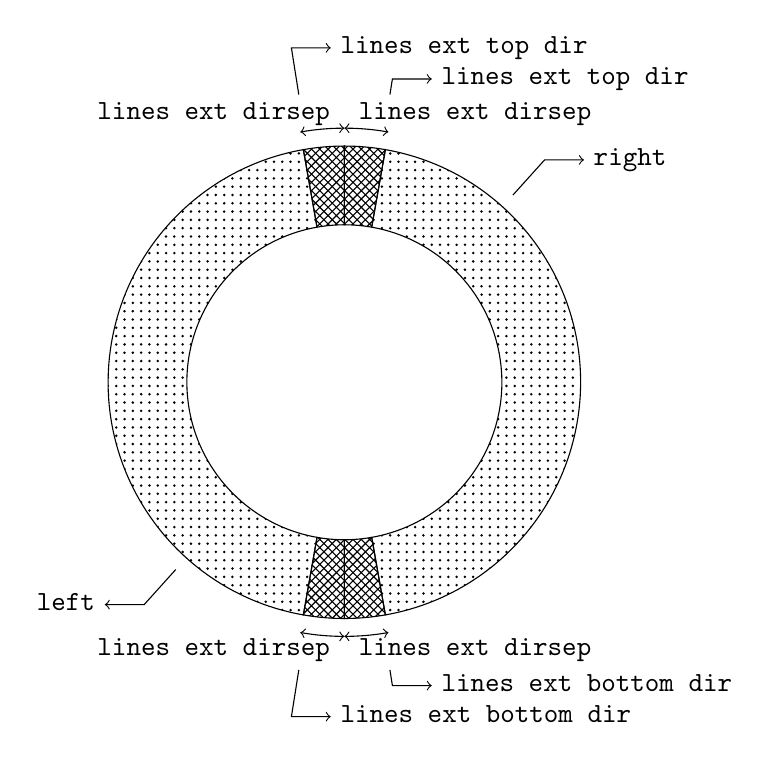
\begin{tikzpicture}[font=\ttfamily]
\def\WClinesextdirsep{10}
\wheelchart[
    data{1,6}=lines ext top dir,
    data{2}=right,
    data{3,4}=lines ext bottom dir,
    data{5}=left,
    data angle pos=\WClistdap,
    data sep=0,
    inner data angle pos{1,4}=0.1,
    inner data angle pos{3,6}=0.9,
    inner data pos=1,
    inner data sep=0.4,
    inner data style={anchor=\WClistia},
    lines=0.6,
    lines{1,3}=0.2,
    lines angle pos=\WClistdap,
    lines ext,
    lines ext dirsep=\WClinesextdirsep,
    lines sep{list}={0.7,0.2,0.7},
    lines style=->,
    slice{1,3,4,6}={
        arc=<->,
        inner data=lines ext dirsep,
        value=\WClinesextdirsep
    },
    slices style={
        draw,
        pattern=\WClistpattern
    },
    total count=6,
    value{2,5}=180-2*\WClinesextdirsep,
    WClistdap={0.9,0.2,0.1},
    WClistia={west,east},
    WClistpattern={
        crosshatch,dots,crosshatch
    }
]{}
\end{tikzpicture}
\end{codeexample}
\end{key}
\begin{key}{/wheelchart/lines ext dirsep=\marg{angle} (initially 0)}
This key determines half the angle in degrees of the segment to which the keys |lines ext bottom dir| and |lines ext top dir| apply.
\end{key}
\begin{key}{/wheelchart/lines ext fixed=\opt{\meta{boolean}} (default true, initially false)}
If true, the line between the wheelchart and the contents of the key |data| will be extended horizontally till the $x$ coordinate determined by the keys |lines ext fixed left| and |lines ext fixed right|.
\end{key}
\begin{key}{/wheelchart/lines ext fixed left=\marg{value}}
\end{key}
\begin{key}{/wheelchart/lines ext fixed right=\marg{value}}
If |lines ext fixed| is true, the lines are extended horizontally initially to the right till the $x$ coordinate $\text{|outer radius|}+\text{|lines sep|}+\text{|lines|}+\text{|lines ext|}$ and to the left till the opposite of this $x$ coordinate. This can be overruled by giving an explicit value to the key |lines ext fixed left| and/or |lines ext fixed right|.
\end{key}
\begin{key}{/wheelchart/lines ext left anchor=\marg{anchor} (initially mid east)}
\end{key}
\begin{key}{/wheelchart/lines ext right anchor=\marg{anchor} (initially mid west)}
\begin{table}[ht]
\centering
\begin{tabular}{ll}
The direction in which the lines between the & \\
wheelchart and the contents of the key |data| will & \\
be extended horizontally if $\text{|lines ext|}\neq 0$ & Anchor of the key |data|\\\hline
left & value of the key |lines ext left anchor|\\
right & value of the key |lines ext right anchor|\\
\end{tabular}
\caption{Anchor of the key \texttt{data} in the case that $\text{\ttfamily lines ext}\neq 0$.}\label{tableanchorofthekeydatainthecasethatlinesextdifferentfromzero}
\end{table}
\end{key}
\begin{key}{/wheelchart/lines ext top dir=\mchoice{left,right} (initially right)}
\end{key}
\begin{key}{/wheelchart/lines pos=\marg{value} (initially 1)}
\end{key}
\begin{key}{/wheelchart/lines sep=\marg{value} (initially 0.2)}
These keys are similar to the corresponding keys for |data| but determine the start point of the lines.
\end{key}
\begin{stylekey}{/wheelchart/lines style=\marg{options} (initially \normalfont empty)}
This key accepts a list of keys which will be applied to the lines drawn by the key |lines|.
\begin{codeexample}[width=10cm,preamble={\usepackage{siunitx}
\usetikzlibrary{decorations.markings}}]
\begin{tikzpicture}
\wheelchart[
    data=\WCperc,
    data angle pos{4}=0.2,
%    data style={outer xsep=4pt},
    legend columns=2,
    legend row={\tikz\fill[\WCvarB] (0,0) circle[radius=0.15]; & \WCvarC & $\WCvarA$},
    legend={
        \node[anchor=north,draw,rounded corners,thick] at (0,-4.5) {%
            \begin{tabular}{*{2}{l@{ }lr}}%
            \WClegend%
            \end{tabular}%
        };
    },
    lines=0.5,
    lines ext=1,
    lines ext bottom dir=left,
    lines ext dirsep=1,
    lines ext fixed,
    lines ext top dir=right,
    lines sep=0,
    lines style={
        \WCvarB,
        postaction=decorate,
        decoration={
            markings,
            mark=at position 1 with {\fill[\WCvarB] (0,0) circle[radius=0.15];}
        }
    },
    start angle=331.2
]{\exampleforthismanual}
\wheelchart[
    data=,
    radius={1.5}{2},
    slices style=\WCvarB!70,
    start angle=331.2
]{\exampleforthismanual}
\end{tikzpicture}
\end{codeexample}
\begin{codeexample}[width=10cm]
\begin{tikzpicture}
\wheelchart[
    data sep=0,
    data style={
        inner sep=0pt,
        shift={(0,0.1)}
    },
    lines=0.5,
    lines ext=1.2,
    lines ext bottom dir=right,
    lines ext dirsep=1,
    %lines ext fixed,
    lines ext left anchor=base west,
    lines ext right anchor=base east,
    lines ext top dir=left,
    lines pos=0.5,
    lines sep=0,
    %lines style=\WCvarB,
    start angle=331.2
]{\exampleforthismanual}
\end{tikzpicture}
\end{codeexample}
\begin{codeexample}[width=10cm,preamble={\usetikzlibrary{decorations.markings}}]
\begin{tikzpicture}
\wheelchart[
    data=\WCvarC: \WCvarA,
    data angle shift=\WCvarG,
    data sep=0,
    data style={draw=\WCvarB,fill=\WCvarB!20},
    lines=1.5,
    lines ext=1,
    lines sep=-1,
    lines style={
        Black,
        postaction=decorate,
        decoration={
            markings,
            mark=at position 0 with {\fill[Black] (0,0) circle[radius=0.15];}
        }
    },
    pie,
    start angle=331.2
]{\exampleforthismanual}
\end{tikzpicture}
\end{codeexample}
\end{stylekey}
\begin{key}{/wheelchart/middle=\marg{text} (initially \normalfont empty)}
This key contains the \meta{text} which will be placed at the center of the wheelchart. The \meta{text} is placed in a node. The style of this node is given as follows. First, the option |align=center| is given. Thereafter, the style of the key |middle style| is added.
\end{key}
\begin{stylekey}{/wheelchart/middle fill=\marg{options} (initially \normalfont empty)}
If this key is set then the middle of the wheelchart will be filled with this style. This key does \emph{not} apply if a plot is used.
\begin{codeexample}[width=10cm]

\begin{tikzpicture}
\wheelchart[
    counterclockwise,
    middle fill={
        Green,
        draw=Red,
        ultra thick
    },
    radius={0.8*\WCcount}
        {0.4+0.8*\WCcount},
    slices style={
        draw=Blue,
        fill=none,
        ultra thick
    },
    start angle=0,
    total angle=300,
    total count=4
]{}
\end{tikzpicture}
\end{codeexample}
\end{stylekey}
\begin{stylekey}{/wheelchart/middle style=\marg{options} (initially \normalfont empty)}
This key accepts a list of keys which will be applied to the node where the contents of the key |middle| is placed.
\end{stylekey}
\begin{key}{/wheelchart/name=\marg{name} (initially wheelchart@name)}
This key defines the \meta{name} of the |local bounding box| around the wheelchart.
\end{key}
\begin{key}{/wheelchart/outer plot=\marg{code}}
This key is similar to the key |inner plot| but determines the outer parts of the slices of the wheelchart.
\begin{codeexample}[]
\begin{tikzpicture}
\wheelchart[
    inner plot={{#1}:{#2+0.2*(cos(#1*\WCtotalcount)+1)}},
    outer plot={{#1}:{#2+0.2*(cos(#1*\WCtotalcount*2)+1)}}
]{\exampleforthismanual}
\end{tikzpicture}
\end{codeexample}
\begin{codeexample}[]

\begin{tikzpicture}
\wheelchart[
    arc data=\WCvarC,
    arc data pos=0.5,
    data=,
    domain=0:450,
    inner plot={
        {int((#1)/180)*5+(0.5-((-1)^Mod(int((#1)/180),2))*2.5)*cos(#1)},
        {(2.5-((-1)^Mod(int((#1)/180),2))*0.5)*sin(#1)}
    },
    outer plot={
        {int((#1)/180)*5+(-0.5-((-1)^Mod(int((#1)/180),2))*2.5)*cos(#1)},
        {(2.5+((-1)^Mod(int((#1)/180),2))*0.5)*sin(#1)}
    },
    value=1
]{\exampleforthismanual}
\end{tikzpicture}
\end{codeexample}
\end{key}
\begin{stylekey}{/wheelchart/outer plot style=\marg{options} (initially \normalfont empty)}
This key accepts a list of keys which will be applied to the plot determined by the key |outer plot|.
\end{stylekey}
\begin{key}{/wheelchart/outer radius=\marg{value} (initially 3)}
The \meta{value} of this key defines the outer radius of the wheelchart.
\end{key}
\begin{key}{/wheelchart/parse=\mchoice{pgfmath,l3fp} (initially pgfmath)}
\begin{description}
\item[\texttt{pgfmath}] In this case, the values of applicable keys will be parsed with |\pgfmathparse|.
\item[\texttt{l3fp}] In this case, the values of applicable keys will be parsed with |\fp_eval:n|.
\end{description}
\end{key}
\begin{key}{/wheelchart/perc precision=\marg{number} (initially 0)}
This key defines the number of decimals up to which the percentage in the macros |\WCperc| and |\WCpercentagerounded| are rounded.
\end{key}
\begin{key}{/wheelchart/pie=\opt{\meta{boolean}} (default true, initially false)}
If true, the inner radius of the wheelchart is set to |0|.
\end{key}
\begin{key}{/wheelchart/plot=\marg{code}}
This key sets |inner plot| and |outer plot|.

Since the \emph{let operation} from the \tikzname{} library |calc| is used, it is not possible to use the variable names |\n|, |\p|, |\x| and |\y| inside the \meta{code}.

Note that positions depend on the |domain| and \emph{not} on the length of the |plot|. For example below, |data angle pos=0.5|. The corresponding value of the |domain| is $1$ which gives the $x$ coordinate $1$ which is \emph{not} in the middle of the plot. Whereas |wheel data angle pos=sqrt(2)/2|. The corresponding value of the |domain| is $\sqrt{2}$ which gives the $x$ coordinate $2$ which is in the middle of the plot.
\begin{codeexample}[width=10cm]

\begin{tikzpicture}
\wheelchart[
    domain=0:2,
    plot={{(#1)^2},{#2}},
    wheel data=text B,
    wheel data angle pos=sqrt(2)/2
]{1/BrickRed/text A}
\end{tikzpicture}
\end{codeexample}
\begin{codeexample}[width=10cm]
\begin{tikzpicture}
\wheelchart[
    plot={{#1}:{0.5*(sin(#1*3)+1)+#2}}
]{\exampleforthismanual}
\end{tikzpicture}
\end{codeexample}
\begin{codeexample}[]

\begin{tikzpicture}
\wheelchart[
    domain=0:720,
    gap polar=5,
    plot={{#1*3.5/180},{sin(#1)-#2}},
    radius={0}{2},
    value=1,
    wheel data=\WCcount,
    wheel data pos=0.5
]{\exampleforthismanual}
\end{tikzpicture}
\end{codeexample}
\begin{codeexample}[width=10cm]

\begin{tikzpicture}
\wheelchart[
    arc data=\WCvarC,
    arc data dir={\WCmidangle<180?-1:1},
    arc data pos=0.5,
    data=,
    domain=0:900,
    plot={{#1}:
        {(((#1)*pi/180+15)^2-1)/300
            +(#2)-0.25}},
    radius={0}{0.5},
    slices arrow={1}{0},
    value=sqrt(3+\WCcount*pi*(pi+6)/7)-
        sqrt(3+(\WCcount-1)*pi*(pi+6)/7)
]{\exampleforthismanual}
\end{tikzpicture}
\end{codeexample}
\begin{codeexample}[]
\begin{tikzpicture}
\pgfkeys{
    /wheelchart,
    gap,
    radius={1.3}{2},
    start angle=180*(1-2/\WCtotalcount),
    value=1
}
\wheelchart[
    plot={{#1}:{(#2)*cos(180/\WCtotalcount)/cos(Mod(#1,{360/\WCtotalcount})-180/\WCtotalcount)}}
]{\exampleforthismanual}
\wheelchart[
    at={(8,0)},
    slices inner arrow={-cot(90*(1-2/\WCtotalcount))}{0},
    slices outer arrow={cot(90*(1-2/\WCtotalcount))}{0}
]{\exampleforthismanual}
\end{tikzpicture}
\end{codeexample}
\end{key}
\begin{stylekey}{/wheelchart/plot style=\marg{options} (initially \normalfont empty)}
This key sets |inner plot style| and |outer plot style|.
\end{stylekey}
\begin{key}{/wheelchart/radius=\marg{inner radius}\marg{outer radius}}
This key defines the inner and outer radius of the wheelchart.
\begin{codeexample}[width=10cm]
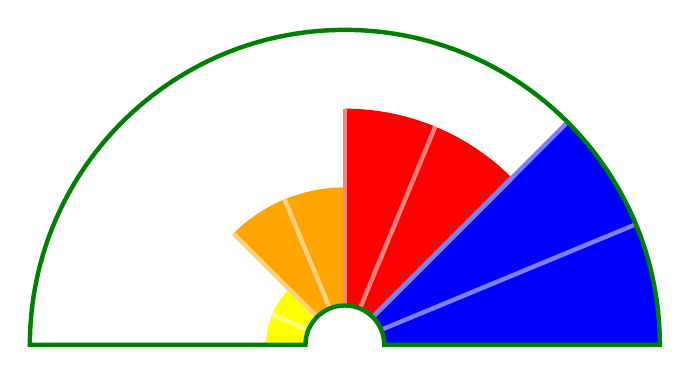
\begin{tikzpicture}
\wheelchart[
    contour={Green,ultra thick},
    data=,
    radius={0.5}{\WCcount},
    slices style=\WCvarA,
    start angle=180,
    total angle=180,
    value=2,
    wheel lines={\WCvarA!50,ultra thick}
]{Yellow,Orange,Red,Blue}
\end{tikzpicture}
\end{codeexample}
\end{key}
\begin{key}{/wheelchart/samples=\marg{number} (initially 25)}
This key determines the \meta{number} of samples used in the plots.
\end{key}
\begin{key}{/wheelchart/separator columns=\marg{delimiter} (initially /)}
\end{key}
\begin{key}{/wheelchart/separator rows=\marg{delimiter} (initially ,)}
The \meta{wheelchart data} in the command |\wheelchart| is a list in which the items are separated by the value of the key |separator rows|. Each item in this list corresponds to one slice of the wheelchart and consists of data separated by the value of the key |separator columns|.
\end{key}
\begin{key}{/wheelchart/slices=\marg{path}}
If this key is set then the shape of the slices of the wheelchart is defined by \meta{path}.
\begin{codeexample}[width=10cm]

\begin{tikzpicture}
\wheelchart[
    radius={2.7}{3.1},
    slices={(0,-0.3)--(0.3,0)--(0,0.3)
        --cycle;},
    value=1
]{\exampleforthismanual}
\wheelchart[
    data=,
    value=1
]{\exampleforthismanual}
\wheelchart[
    data=,
    radius={2}{2},
    slices={(0,0) circle[radius=0.4];},
    slices style=White,
    value=1
]{\exampleforthismanual}
\wheelchart[
    data=,
    radius={2}{2},
    slices={(0,0) circle[radius=0.3];},
    value=1,
    wheel data=\WCcount
]{\exampleforthismanual}
\end{tikzpicture}
\end{codeexample}
In the following example, a |;| is placed at the beginning of the argument for the key |slices| because there is no path to be filled. Thereafter, a node is placed still within the argument for the key |slices|.
\begin{codeexample}[width=10cm]
\begin{tikzpicture}
\wheelchart[
    data=,
    radius={3.5}{3.5},
    slices={;\node[
        bottom color=\WCvarB!60,
        top color=\WCvarB!10,
        circle,
        draw=gray,
        minimum width=2.5cm
    ] (WCslice\WCcount)
        {\WCcount: \WCvarC};},
    slices style={},
    start half,
    value=1
]{\exampleforthismanual}
\foreach\n in {1,...,7}{
\pgfmathsetmacro{\k}{int(Mod(\n,7)+1)}
\draw[->,line width=2pt] (WCslice\n)
    to[bend left=10] (WCslice\k);
}
\end{tikzpicture}
\end{codeexample}
\end{key}
\begin{key}{/wheelchart/slices angle pos=\marg{value} (initially 0.5)}
\end{key}
\begin{key}{/wheelchart/slices angle shift=\marg{angle} (initially 0)}
These keys determine the position of the slices if the key |slices| is used similar as the corresponding keys for the key |data|.
\end{key}
Below we list some keys to modify the shape of the slices. These keys only affect the shape of the slices and \emph{not} the computation of the inner and outer plot. In particular, these keys do \emph{not} affect the placement of |arc data|, |data|, |inner data|, |lines|, |wheel data| and |wheel lines|. If this placement should be changed then the keys |inner plot| and |outer plot| can be used.
\begin{key}{/wheelchart/slices arc=\marg{value 1}\marg{value 2}}
This key sets |slices end arc| and |slices start arc| but uses the opposite of \meta{value 1} for |slices start arc|.
\begin{codeexample}[width=10cm]
\begin{tikzpicture}
\wheelchart[
    slices arc={1}{0},
    wheel data=\WCcount,
    wheel data angle pos=1,
    wheel data pos=0.5,
    wheel data style={
        circle,
        fill=\WCvarB!50
    }
]{\exampleforthismanual}
\end{tikzpicture}
\end{codeexample}
\begin{codeexample}[width=10cm]
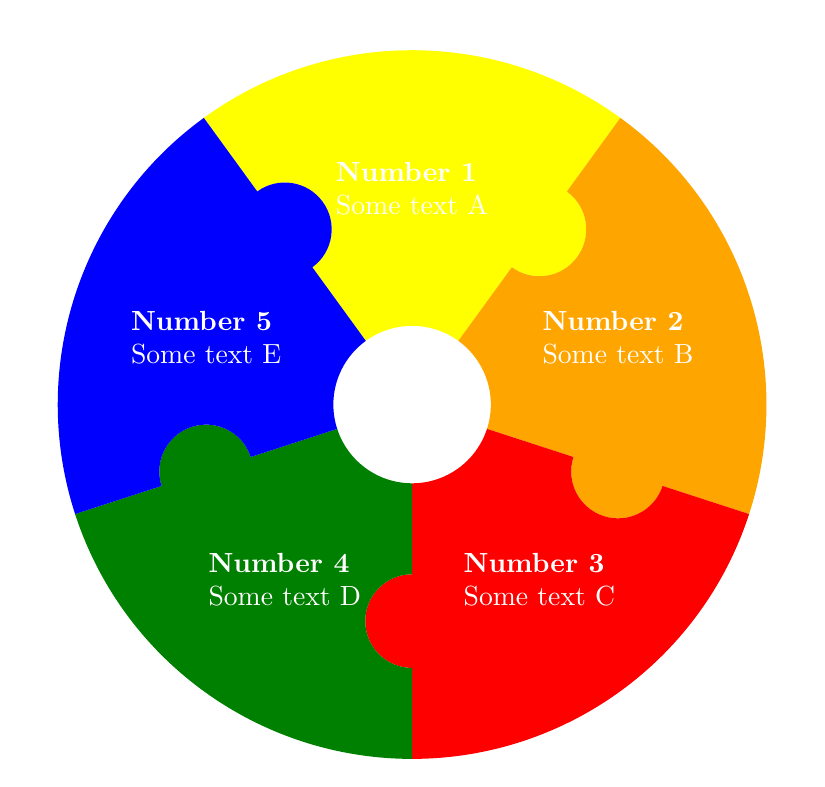
\begin{tikzpicture}
\wheelchart[
    data=,
    radius={1}{4.5},
    slices arc={1}{0.66},
    slices style=\WCvarA,
    start half,
    value=1,
    wheel data={%
        \textbf{Number \WCcount}\\%
        \WCvarB%
    },
    wheel data pos=0.5,
    wheel data style=White
]{%
    Yellow/Some text A,
    Orange/Some text B,
    Red/Some text C,
    Green/Some text D,
    Blue/Some text E%
}
\end{tikzpicture}
\end{codeexample}
\end{key}
\begin{key}{/wheelchart/slices arc inner end=\opt{\meta{boolean}} (default true, initially false)}
If true then the keys |slices end arc|, |slices inner arc| and |slices start arc| are set such that the inner part and the end of each of the slices of the wheelchart form one arc and such that the start has the opposite curvature as the end.
\begin{codeexample}[width=10cm]
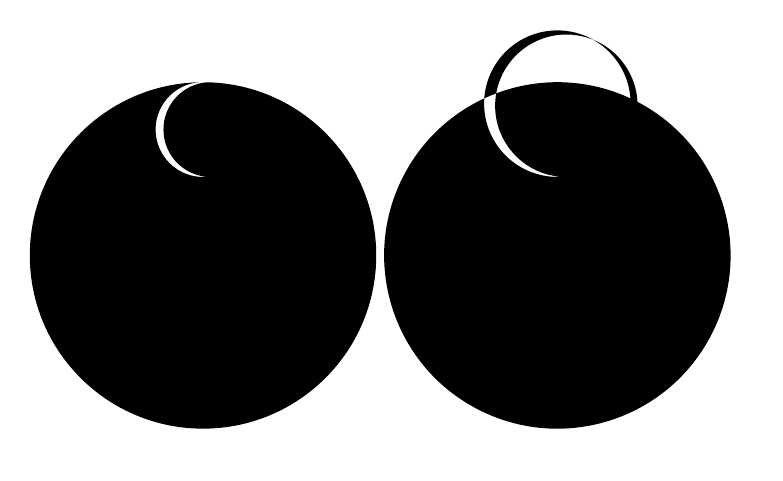
\begin{tikzpicture}[font=\scriptsize]
\foreach\a/\x in {0/0,45/4.5}{
\wheelchart[
    at={(\x,0)},
    data=,
    gap,
    radius={1}{2.2},
    slices arc inner end,
    slices outer angle shift=\a,
    value=1,
    wheel data=\WCvarC,
    wheel data angle pos=0.6
]{\exampleforthismanual}
}
\end{tikzpicture}
\end{codeexample}
\end{key}
\begin{key}{/wheelchart/slices arc inner end start=\opt{\meta{boolean}} (default true, initially false)}
If true then the keys |slices end arc|, |slices inner arc| and |slices start arc| are set such that the inner part and the end of each of the slices of the wheelchart form one arc and such that the start has the same curvature as the end.
\begin{codeexample}[]
\begin{tikzpicture}
\foreach\a/\x in {-60/0,0/4.5,60/10}{
\wheelchart[
    at={(\x,0)},
    radius={0.66}{2},
    slices arc inner end start,
    slices inner angle shift=\a,
    slices style={fill=none,draw=Turquoise,ultra thick},
    total count=20
]{}
}
\end{tikzpicture}
\end{codeexample}
\end{key}
\begin{key}{/wheelchart/slices arc inner start=\opt{\meta{boolean}} (default true, initially false)}
If true then the keys |slices end arc|, |slices inner arc| and |slices start arc| are set such that the inner part and the start of each of the slices of the wheelchart form one arc and such that the end has the opposite curvature as the start.
\begin{codeexample}[width=10cm]
\begin{tikzpicture}
\wheelchart[
    middle={%
        slices arc\\%
        inner start,\\%
        slices inner\\%
        angle shift=90%
    },
    middle style={font=\ttfamily},
    slices arc inner start,
    slices inner angle shift=90
]{%
    1/Goldenrod/,
    1/Mahogany/,
    1/JungleGreen/,
    1/RoyalBlue/%
}
\end{tikzpicture}
\end{codeexample}
\end{key}
\begin{key}{/wheelchart/slices arc inner start end=\opt{\meta{boolean}} (default true, initially false)}
If true then the keys |slices end arc|, |slices inner arc| and |slices start arc| are set such that the inner part and the start of each of the slices of the wheelchart form one arc and such that the end has the same curvature as the start.
\begin{codeexample}[width=10cm]
\begin{tikzpicture}
\wheelchart[
    data=,
    gap polar=5,
    middle={%
        slices arc\\%
        inner start end%
    },
    middle style={font=\ttfamily},
    slices arc inner start end,
    value=1,
    wheel data=\WCvarC,
    wheel data pos=0.4
]{\exampleforthismanual}
\end{tikzpicture}
\end{codeexample}
\end{key}
\begin{key}{/wheelchart/slices arc match=\marg{arg 1}\marg{num 1}\marg{num 2}\marg{num 3}\marg{arg 2}\marg{arg 3}\marg{arg 4}}
This key modifies the shape of the slices according to the $7$ arguments.

Here, \meta{arg 1} must be |end|, |inner|, |outer| or |start| and \meta{arg 2}, \meta{arg 3} and \meta{arg 4} must be |inner end|, |inner start|, |outer end| or |outer start|. For example, the key |slices arc inner end| sets |slices arc match={inner}{1}{-1}{1}{inner end}{inner start}{outer end}|.
\begin{codeexample}[width=10cm]
\begin{tikzpicture}
\foreach\a/\b/\x in
    {end/1/0,inner/-1/4.8}{
\wheelchart[
    at={(\x,0)},
    radius={0.66}{2},
    slices arc match=
        {\a}{\b}{1}{1}{inner end}
        {inner start}{outer end},
    slices inner angle shift=60,
    slices style={
        fill=none,
        draw=Turquoise
    },
    total count=20
]{}
}
\end{tikzpicture}
\end{codeexample}
\end{key}
\begin{key}{/wheelchart/slices arc outer end=\opt{\meta{boolean}} (default true, initially false)}
If true then the keys |slices end arc|, |slices outer arc| and |slices start arc| are set such that the outer part and the end of each of the slices of the wheelchart form one arc and such that the start has the opposite curvature as the end.
\end{key}
\begin{key}{/wheelchart/slices arc outer end start=\opt{\meta{boolean}} (default true, initially false)}
If true then the keys |slices end arc|, |slices outer arc| and |slices start arc| are set such that the outer part and the end of each of the slices of the wheelchart form one arc and such that the start has the same curvature as the end.
\begin{codeexample}[width=10cm]
\begin{tikzpicture}
\wheelchart[
    data=,
    gap polar=5,
    middle={%
        slices arc\\%
        outer end start%
    },
    middle style={font=\ttfamily},
    slices arc outer end start,
    value=1,
    wheel data=\WCvarC
]{\exampleforthismanual}
\end{tikzpicture}
\end{codeexample}
\end{key}
\begin{key}{/wheelchart/slices arc outer start=\opt{\meta{boolean}} (default true, initially false)}
If true then the keys |slices end arc|, |slices outer arc| and |slices start arc| are set such that the outer part and the start of each of the slices of the wheelchart form one arc and such that the end has the opposite curvature as the start.
\begin{codeexample}[width=10cm]
\begin{tikzpicture}
\wheelchart[
    data=,
    gap=0.1,
    slices arc inner start,
    slices arc outer start,
    slices style={
        \WCvarB!50,
        draw=\WCvarB,
        ultra thick
    },
    value=1,
    wheel data=\WCcount,
    wheel data pos=0.8
]{\exampleforthismanual}
\end{tikzpicture}
\end{codeexample}
\begin{codeexample}[]
\begin{tikzpicture}
\foreach\a/\x in {0/0,45/5,90/10}{
\wheelchart[
    at={(\x,0)},
    data=,
    gap,
    radius={0.66}{2},
    slices arc outer start,
    slices outer angle shift=\a,
    value=1
]{\exampleforthismanual}
}
\end{tikzpicture}
\end{codeexample}
\end{key}
\begin{key}{/wheelchart/slices arc outer start end=\opt{\meta{boolean}} (default true, initially false)}
If true then the keys |slices end arc|, |slices outer arc| and |slices start arc| are set such that the outer part and the start of each of the slices of the wheelchart form one arc and such that the end has the same curvature as the start.
\end{key}
\begin{key}{/wheelchart/slices arrow=\marg{value 1}\marg{value 2}}
This key is similar to the key |slices arc| but draws an arrow.
\begin{codeexample}[width=10cm]
\begin{tikzpicture}
\wheelchart[
    gap=0.3,
    slices arrow={1}{-1}
]{\exampleforthismanual}
\end{tikzpicture}
\end{codeexample}
\end{key}
\begin{key}{/wheelchart/slices end arc=\marg{value 1}\marg{value 2}}
This key determines the end of the slice.

The effect of \meta{value 1} and \meta{value 2} is shown in the figure and the table below.

If $\text{\meta{value 1}}>0$ then the arc points outwards the slice. If $\text{\meta{value 1}}<0$ then the arc points inwards the slice. Here, outwards and inwards are relative to the orientation of the four-sided polygon formed by the points whose coordinates are determined by the inner and outer radius of the first slice and the start angle and the angle at the inverse of the key |samples| between the start angle and the end angle of the first slice. If the start angle and the end angle of the first slice are equal then the end angle of the last slice is used instead. If this test is inconclusive then the orientation is set according to the key |counterclockwise|.

If $\text{\meta{value 1}}=0$ then a line segment is drawn.

If \meta{value 1} and \meta{value 2} are negative then an arc is drawn which behaves the same as an arc with $\text{\meta{value 2}}=0$ and such that its radius matches the radius of the arc corresponding to setting \meta{value 1} to its opposite. This is illustrated in the table below.
\begin{center}
\begin{tikzpicture}[scale=3]
\wheelchart[
    slices end arc={2}{0.5},
    slices style={
        fill=none,
        draw=Cyan,
        ultra thick
    },
    xbar={1}{1}
]{1//}
\draw[<->] (1,0.5)--(1.5,0.5) node[below,midway] {$a$};
\draw[<->] (1,0.5)--(1,0.75) node[left,midway] {$b$};
\draw[<->] (1,0.75)--(1,1) node[left,midway] {$c$};
\draw[<->] (0.75,0.5)--(0.75,1) node[left,midway] {$d$};
\node[right] at (2,0.5) {$\lvert\text{\meta{value 1}}\rvert=\frac{a}{b},\ \lvert\text{\meta{value 2}}\rvert=\frac{c}{d}$};
\end{tikzpicture}

\newcommand{\exampleslicesarc}[2]{%
\begin{tikzpicture}[baseline={(0,0.5)}]
\ifdim #1 pt<0pt
\ifdim #2 pt<0pt
\edef\r{\fpeval{0.25*((#2)-1)*(1/(#1)+(#1))}}
\wheelchart[
    at={({1.5+sqrt((\r)^2-0.25)-(#1)*0.5*(1-(#2))-\r},0)},
    slices start arc={-(#1)}{#2},
    slices style={
        fill=none,
        draw=Goldenrod,
        ultra thick
    },
    xbar={0.5}{1}
]{1//}
\fi
\fi
\wheelchart[
    slices end arc={#1}{#2},
    slices style={
        fill=none,
        draw
    },
    xbar={1.5}{1}
]{1//}
\useasboundingbox ($(current bounding box.south west)-(2pt,2pt)$) rectangle ($(current bounding box.north east)+(2pt,2pt)$);
\end{tikzpicture}%
}
\newcommand{\exampleslicesarcrow}[1]{$\text{\meta{value 1}}=#1$ & \exampleslicesarc{#1}{-0.5} & \exampleslicesarc{#1}{0} & \exampleslicesarc{#1}{0.5}\\}
\begin{tabular}{l|lll}
 & $\text{\meta{value 2}}=-0.5$ & $\text{\meta{value 2}}=0$ & $\text{\meta{value 2}}=0.5$\\\hline
\exampleslicesarcrow{2}
\exampleslicesarcrow{1}
\exampleslicesarcrow{0}
\exampleslicesarcrow{-1}
\exampleslicesarcrow{-2}
\end{tabular}
\end{center}
\begin{codeexample}[width=10cm]
\begin{tikzpicture}
\wheelchart[
    for loop start={
        \definecolor{WCcolor}{wave}{
        \fpeval{380+(\WCcount-1)*
        340/(\WCtotalcount-1)}}
    },
    gap polar=180/\WCtotalcount,
    radius={1.5}{3},
    slices end arc={-0.6}{0},
    slices start arc={1.2}{0},
    slices style=WCcolor,
    total count=20
]{}
\end{tikzpicture}
\end{codeexample}
\end{key}
\begin{key}{/wheelchart/slices end arrow=\marg{value 1}\marg{value 2}}
This key is similar to the key |slices end arc| but draws an arrow.
\end{key}
\begin{key}{/wheelchart/slices end to=\marg{value 1}\marg{value 2}}
This key sets the |to| path operation for the end of the slice. The angle at the inner side is determined by \meta{value 1} and the angle at the outer side is determined by \meta{value 2}.
\end{key}
\begin{key}{/wheelchart/slices inner angle reduce=\marg{angle}}
This key sets |slices inner end angle shift| to $-\text{\meta{angle}}$ and |slices inner start angle shift| to \meta{angle}.
\end{key}
\begin{key}{/wheelchart/slices inner angle shift=\marg{angle}}
This key sets |slices inner end angle shift| and |slices inner start angle shift| to \meta{angle}.
\begin{codeexample}[width=10cm]
\begin{tikzpicture}
\wheelchart[
    data=,
    middle={%
        slices inner\\%
        angle shift=90%
    },
    middle style={font=\ttfamily},
    slices inner angle shift=90
]{\exampleforthismanual}
\end{tikzpicture}
\end{codeexample}
\begin{codeexample}[width=10cm]
\begin{tikzpicture}
\wheelchart[
    data=,
    gap,
    radius={1}{3},
    slices arc={0.5}{0},
    slices inner angle shift=45,
    value=1,
    wheel data=\WCvarC,
    wheel data angle pos=0.8
]{\exampleforthismanual}
\end{tikzpicture}
\end{codeexample}
\begin{codeexample}[]
\begin{tikzpicture}
\foreach\a/\x in {-60/0,0/5.6,60/10}{
\wheelchart[
    at={(\x,0)},
    radius={0.66}{2},
    slices arc inner start,
    slices inner angle shift=\a,
    slices style={fill=\WClistcolors},
    total count=40,
    WClistcolors={RedOrange,none}
]{}
}
\end{tikzpicture}
\end{codeexample}
\begin{codeexample}[width=10cm]
\begin{tikzpicture}[font=\small]
\pgfkeys{
    /wheelchart,
    data=,
    inner data=\WCcount,
    inner data pos=0.1,
    inner data sep=0,
    radius={1}{2.4},
    slices inner angle shift=
        90-180/\WCtotalcount,
    slices inner arc={0}{0},
    value=1,
    wheel data=\WCvarC
}
\wheelchart{\exampleforthismanual}
\wheelchart[
    at={(4.8,0)},
    slices outer arc={0}{0},
    wheel data pos=0.58
]{\exampleforthismanual}
\end{tikzpicture}
\end{codeexample}
\end{key}
\begin{key}{/wheelchart/slices inner arc=\marg{value 1}\marg{value 2}}
This key is similar to the key |slices end arc| but sets the inner part of the slice.
\end{key}
\begin{key}{/wheelchart/slices inner arc tangent=\opt{\meta{boolean}} (default true, initially false)}
If true then the key |slices inner arc| is set such that the arc is tangent to the end and start of the slice if possible. Note that this is not possible for all settings for keys such as |plot| and |slices inner angle shift|.
\begin{codeexample}[width=10cm]
\begin{tikzpicture}
\wheelchart[
    counterclockwise,
    data=,
    gap=0.1,
    middle=slices inner\\arc tangent,
    middle style={font=\ttfamily},
    slices inner arc tangent,
    slices style={
        draw=\WCvarB,
        fill=\WCvarB!50,
        ultra thick
    },
    value=1
]{\exampleforthismanual}
\end{tikzpicture}
\end{codeexample}
\end{key}
\begin{key}{/wheelchart/slices inner arrow=\marg{value 1}\marg{value 2}}
This key is similar to the key |slices end arrow| but sets the inner part of the slice.
\begin{codeexample}[width=10cm]
\begin{tikzpicture}
\def\n{10}
\wheelchart[
    radius={0}{1.5},
    slices outer arrow={cot(180/\n)}{0},
    slices style{list}={
        BurntOrange,RedOrange
    },
    total count=\n
]{}
\wheelchart[
    radius={3*cos(180/\n)}
        {3*cos(180/\n)},
    slices inner arrow={cot(360/\n)}{0},
    slices outer arrow={cot(360/\n)}{0},
    slices style{list}={
        Dandelion,Goldenrod
    },
    start half,
    total count=\n
]{}
\end{tikzpicture}
\end{codeexample}
\end{key}
\begin{key}{/wheelchart/slices inner end angle shift=\marg{angle} (initially 0)}
The end angle of the inner part of the slice will be modified such that the angle between the end and the inner part of the slice is shifted with \meta{angle} (taking into account the key |counterclockwise|). The behavior of this key depends on whether a plot is used.
\end{key}
\begin{key}{/wheelchart/slices inner start angle shift=\marg{angle} (initially 0)}
This key is similar to the key |slices inner end angle shift| but modifies the start angle of the inner part of the slice.
\end{key}
\begin{key}{/wheelchart/slices inner to=\marg{value 1}\marg{value 2}}
This key sets the |to| path operation for the inner part of the slice. The angle at the start is determined by \meta{value 1} and the angle at the end is determined by \meta{value 2}.
\end{key}
\begin{key}{/wheelchart/slices outer angle reduce=\marg{angle}}
This key sets |slices outer end angle shift| to $-\text{\meta{angle}}$ and |slices outer start angle shift| to \meta{angle}.
\begin{codeexample}[width=10cm]
\begin{tikzpicture}
\wheelchart[
    data=,
    inner data=\WCcount,
    inner data style={
        circle,
        fill=white
    },
    slices inner arrow={1}{0},
    slices outer angle reduce=
        180/\WCtotalcount,
    slices outer arrow={0}{0},
    value=1,
    wheel data=\WCvarC,
    wheel data style={
        rotate=\WCmidangle-90
    }
]{\exampleforthismanual}
\end{tikzpicture}
\end{codeexample}
\end{key}
\begin{key}{/wheelchart/slices outer angle shift=\marg{angle}}
This key sets |slices outer end angle shift| and |slices outer start angle shift| to \meta{angle}.
\begin{codeexample}[width=10cm]
\begin{tikzpicture}[looseness=2]
\wheelchart[
    data=,
    inner data={\Large\WCcount},
    inner data pos=1.1,
    radius={1}{3},
    slices arc inner end,
    slices outer angle shift=80,
    slices outer to={80}{80},
    slices style={
        bottom color=\WCvarB,
        top color=\WCvarB!80!black,
        shading angle=\WCmidangle-90
    },
    value=1,
    wheel data=\WCvarC,
    wheel data angle pos=0.4,
    wheel data pos=0.8
]{\exampleforthismanual}
\end{tikzpicture}
\end{codeexample}
\end{key}
\begin{key}{/wheelchart/slices outer arc=\marg{value 1}\marg{value 2}}
This key is similar to the key |slices end arc| but sets the outer part of the slice.
\end{key}
\begin{key}{/wheelchart/slices outer arc tangent=\opt{\meta{boolean}} (default true, initially false)}
If true then the key |slices outer arc| is set such that the arc is tangent to the end and start of the slice if possible. Note that this is not possible for all settings for keys such as |plot| and |slices inner angle shift|.
\begin{codeexample}[width=10cm]
\begin{tikzpicture}
\wheelchart[
    data=,
    gap=0.1,
    middle=slices outer\\arc tangent,
    middle style={font=\ttfamily},
    slices outer arc tangent,
    slices style={
        draw=\WCvarB,
        fill=\WCvarB!50,
        ultra thick
    },
    value=1
]{\exampleforthismanual}
\end{tikzpicture}
\end{codeexample}
\end{key}
\begin{key}{/wheelchart/slices outer arrow=\marg{value 1}\marg{value 2}}
This key is similar to the key |slices end arrow| but sets the outer part of the slice.
\begin{codeexample}[width=10cm]
\begin{tikzpicture}[font=\scriptsize]
\foreach\a/\x in
    {1/0,{tan(180/\WCtotalcount)}/5}{
\wheelchart[
    at={(\x,0)},
    data=,
    gap,
    radius={0.66}{2},
    slices outer arrow={\a}{0},
    start half,
    value=1,
    wheel data=\WCvarC
]{\exampleforthismanual}
}
\end{tikzpicture}
\end{codeexample}
\begin{codeexample}[width=10cm]
\begin{tikzpicture}
\pgfkeys{
    /wheelchart,
    data=,
    radius={1}{1.5},
    value=1
}
\wheelchart[
    slices inner arrow={0}{0}
]{\exampleforthismanual}
\wheelchart[
    at={(3.25,0)},
    slices outer arrow={0}{0}
]{\exampleforthismanual}
\wheelchart[
    at={(6.5,0)},
    slices inner arrow={0}{0},
    slices outer arrow={0}{0}
]{\exampleforthismanual}
\end{tikzpicture}
\end{codeexample}
\begin{codeexample}[width=10cm]
\begin{tikzpicture}
\foreach\r/\s/\a in
    {3/0/0.5,2/15/1,1/30/0.7}{
\wheelchart[
    radius={0.5}{\r},
    slices outer arrow={\a}{0},
    slices style={
        fill=\WClistcolors!20,
        draw=\WClistcolors,
        ultra thick,
        double
    },
    start half=\s,
    total count=12,
    WClistcolors={CarnationPink,Orchid}
]{}
}
\end{tikzpicture}
\end{codeexample}
\end{key}
\begin{key}{/wheelchart/slices outer end angle shift=\marg{angle} (initially 0)}
The end angle of the outer part of the slice will be modified such that the angle between the end and the inner (not the outer) part of the slice is shifted with \meta{angle} (taking into account the key |counterclockwise|). The behavior of this key depends on whether a plot is used.
\end{key}
\begin{key}{/wheelchart/slices outer start angle shift=\marg{angle} (initially 0)}
This key is similar to the key |slices outer end angle shift| but modifies the start angle of the outer part of the slice.
\end{key}
\begin{key}{/wheelchart/slices outer to=\marg{value 1}\marg{value 2}}
This key sets the |to| path operation for the outer part of the slice. The angle at the start is determined by \meta{value 1} and the angle at the end is determined by \meta{value 2}.
\begin{codeexample}[width=10cm]
\begin{tikzpicture}[looseness=3]
\wheelchart[
    data=,
    radius={0}{2.5},
    slices arc={0.4}{0},
    slices outer to={70}{70},
    start half,
    value=1,
    wheel data=\WCvarC,
    wheel data pos=1
]{\exampleforthismanual}
\end{tikzpicture}
\end{codeexample}
\end{key}
\begin{key}{/wheelchart/slices pos=\marg{value} (initially 0.5)}
This key determines the position of the slices if the key |slices| is used similar as the corresponding key for the key |data|.
\end{key}
\begin{stylekey}{/wheelchart/slices scope=\marg{options} (initially \normalfont empty)}
This key accepts a list of keys which will be applied to the scope in which the slices of the wheelchart, the wheel lines determined by the key |wheel lines| and the different kinds of data are placed.
\begin{codeexample}[width=10cm]
\begin{tikzpicture}
\wheelchart[
    data=,
    radius={3.9}{4.5},
    slices inner arc={0}{0},
    slices outer angle reduce=5*90/7,
    slices outer arc={0}{0},
    slices scope={
        shift={
            ($(90+\WCmidangle:0.559572)
            +(\WCmidangle:-1.16196)$)
        }
    },
    value=1,
    wheel data=\WCvarC,
    wheel data pos=0,
    wheel data style={
        rotate=\WCmidangle-90
    }
]{\exampleforthismanual}
\end{tikzpicture}
\end{codeexample}
\begin{codeexample}[width=10cm,preamble={\usepackage{siunitx}}]
\begin{tikzpicture}
\wheelchart[
    data=\WCvarC\\%
        \qty{\fpeval{\WCvarA/2}}%
        {\percent},
    radius={0.5}{0.5+0.1*\WCvarA},
    slices inner arc tangent,
    slices outer angle reduce=
        180/\WCtotalcount,
    slices outer arc tangent,
    slices scope={shift={(\WCmidangle:
        {-cos(180/\WCtotalcount)/2})}},
    value=1
]{\exampleforthismanual}
\end{tikzpicture}
\end{codeexample}
\end{stylekey}
\begin{key}{/wheelchart/slices sep=\marg{value} (initially 0)}
This key determines the position of the slices if the key |slices| is used similar as the corresponding key for the key |data|.
\end{key}
\begin{key}{/wheelchart/slices start arc=\marg{value 1}\marg{value 2}}
This key is similar to the key |slices end arc| but sets the start of the slice.
\end{key}
\begin{key}{/wheelchart/slices start arrow=\marg{value 1}\marg{value 2}}
This key is similar to the key |slices end arrow| but sets the start of the slice.
\end{key}
\begin{key}{/wheelchart/slices start to=\marg{value 1}\marg{value 2}}
This key sets the |to| path operation for the start of the slice. The angle at the inner side is determined by \meta{value 1} and the angle at the outer side is determined by \meta{value 2}.
\end{key}
\begin{stylekey}{/wheelchart/slices style=\marg{options} (initially \textbackslash WCvarB)}
This key defines the style of the slices of the wheelchart.
\end{stylekey}
\begin{key}{/wheelchart/slices to=\marg{value 1}\marg{value 2}}
This key sets |slices end to| and |slices start to| but uses the opposite respective values for |slices start to|.
\begin{codeexample}[width=10cm]
\begin{tikzpicture}[looseness=2]
\wheelchart[
    radius={1}{3},
    slices inner angle shift=90,
    slices inner arc={0}{0},
    slices outer to={70}{70},
    slices style{list}={Maroon,Salmon},
    slices to={30}{30},
    total count=6
]{}
\end{tikzpicture}
\end{codeexample}
\end{key}
\begin{stylekey}{/wheelchart/slice\marg{range}=\marg{options} (initially \normalfont empty)}
This key accepts a list of keys from the wheelchart key family. The \meta{range} is mandatory and must be non-empty. It is processed with |\foreach| with the option |parse=true|. Hereafter the elements are processed with |\fp_eval:n|. The \meta{options} will only be applied to a slice if the number of the slice is in the \meta{range}. The \meta{range} only makes sense for a key which is processed for each slice. For example, the \meta{range} does not make sense for the key |middle|.
\end{stylekey}
\begin{key}{/wheelchart/start angle=\marg{angle} (initially 90)}
This key defines the \meta{angle} in degrees at which the first slice of the wheelchart starts.
\end{key}
\begin{key}{/wheelchart/start half=\marg{angle} (default 90)}
This key sets the start angle such that the middle of the first slice of the wheelchart is positioned at \meta{angle} in degrees.
\end{key}
\begin{key}{/wheelchart/title=\marg{text} (initially \normalfont empty)}
This key contains the \meta{text} which will be placed above the wheelchart. The \meta{text} is placed in a node. The $x$ coordinate of this node is the $x$ coordinate of the center of the wheelchart, which is defined by the key |at|. In general, this is \emph{not} the same as the $x$ coordinate of the center of the |local bounding box| around the wheelchart. The $y$ coordinate of this node is at a value determined by the key |title sep| above the north of the |local bounding box| around the wheelchart. The style of this node is given as follows. First, the options |anchor=south,align=center| are given. Thereafter, the style of the key |title style| is added.
\end{key}
\begin{key}{/wheelchart/title left=\marg{text} (initially \normalfont empty)}
This key contains the \meta{text} which will be placed above left of the wheelchart. The \meta{text} is placed in a node. This node is placed at a value determined by the key |title left sep| above the north west of the |local bounding box| around the wheelchart. The style of this node is given as follows. First, the options |anchor=south west,align=left| are given. Thereafter, the style of the key |title left style| is added.
\end{key}
\begin{key}{/wheelchart/title left sep=\marg{value} (initially 0.5)}
The node where the contents of the key |title left| is placed is at \meta{value} above the north west of the |local bounding box| around the wheelchart.
\end{key}
\begin{stylekey}{/wheelchart/title left style=\marg{options} (initially \normalfont empty)}
This key accepts a list of keys which will be applied to the node where the contents of the key |title left| is placed.
\end{stylekey}
\begin{key}{/wheelchart/title sep=\marg{value} (initially 0.5)}
The $y$ coordinate of the node where the contents of the key |title| is placed is at \meta{value} above the north of the |local bounding box| around the wheelchart.
\end{key}
\begin{stylekey}{/wheelchart/title style=\marg{options} (initially \normalfont empty)}
This key accepts a list of keys which will be applied to the node where the contents of the key |title| is placed.
\end{stylekey}
\begin{key}{/wheelchart/total angle=\marg{angle} (initially 360)}
This key defines the total \meta{angle} in degrees of the wheelchart.
\end{key}
\begin{key}{/wheelchart/total count=\marg{number}}
If this key is set then the number of slices of the wheelchart is determined by \meta{number}. Moreover, |\WCvarA| is defined as |1| and |\WCvarB| and |\WCvarC| are defined to be empty.
\begin{codeexample}[width=10cm,preamble={\usepackage{siunitx}}]
\begin{tikzpicture}
\def\n{57}
\wheelchart[
    gap=0.015,
    middle={\Huge\qty{\n}{\percent}},
    slices style=Gray,
    slices style{1,...,\n}=Cyan,
    total count=100
]{}
\end{tikzpicture}
\end{codeexample}
\end{key}
\begin{key}{/wheelchart/triangle proportional area=\marg{width}\marg{height}}
This key configures the plot such that a triangular shape is obtained. The value is proportional to the area and \emph{not} to the height. Moreover, it sets |samples=2| and |wheel data pos=0.5|. The point $(0,0)$ is at the top. This can be shifted with the key |at|.
\begin{codeexample}[width=10cm]
\begin{tikzpicture}
\wheelchart[
    triangle proportional area={5}{4},
    value=1
]{\exampleforthismanual}
\end{tikzpicture}
\end{codeexample}
\end{key}
\begin{key}{/wheelchart/triangle proportional height=\marg{width}\marg{height}}
This key configures the plot such that a triangular shape is obtained. The value is proportional to the height and \emph{not} to the area. Moreover, it sets |samples=2| and |wheel data pos=0.5|. The point $(0,0)$ is at the top. This can be shifted with the key |at|.
\begin{codeexample}[width=10cm]
\begin{tikzpicture}
\wheelchart[
    triangle proportional height={5}{4},
    value=1
]{\exampleforthismanual}
\end{tikzpicture}
\end{codeexample}
\end{key}
\begin{key}{/wheelchart/value=\marg{value} (initially \textbackslash WCvarA)}
This key defines the \meta{value} which corresponds to the size of each slice of the wheelchart.
\end{key}
\begin{key}{/wheelchart/WClist\meta{name}=\marg{list}}
This key locally defines a macro |\WClist|\meta{name} which gives the element in the \meta{list} with as index |\WCcount| modulo the length of the \meta{list}. The \meta{list} is expanded once and processed using a |clist|. In particular, blank arguments are ignored. An empty argument in the \meta{list} can be obtained with |{}|. Items containing a |,| can be obtained by surrounding it with |{| and |}| such as |WClistA={{a,b},{c,d}}|.

If |\def\mylist{a,b,c}| and |WClistA=\mylist| then |\WClistA| gives |a,b,c| for each slice. On the other hand, if |WClistA/.expanded=\mylist| then |\WClistA| alternates between |a|, |b| and |c|.
\end{key}
\begin{key}{/wheelchart/wheel data=\marg{text} (initially \normalfont empty)}
This key contains the \meta{text} which will be placed on top of each slice of the wheelchart. The \meta{text} is placed in a node. The style of this node is given as follows. First, the option |align=left| is given. Thereafter, the style of the key |wheel data style| is added.
\end{key}
\begin{key}{/wheelchart/wheel data angle pos=\marg{value} (initially 0.5)}
\end{key}
\begin{key}{/wheelchart/wheel data angle shift=\marg{angle} (initially 0)}
\end{key}
\begin{key}{/wheelchart/wheel data pos=\marg{value} (initially 0.66)}
\end{key}
\begin{key}{/wheelchart/wheel data sep=\marg{value} (initially 0)}
These keys determine the position of the contents of the key |wheel data| similar as the corresponding keys for the key |data|.
\end{key}
\begin{stylekey}{/wheelchart/wheel data style=\marg{options} (initially \normalfont empty)}
This key accepts a list of keys which will be applied to the node where the contents of the key |wheel data| is placed.
\end{stylekey}
\begin{stylekey}{/wheelchart/wheel lines=\marg{options} (initially \normalfont empty)}
If this key is set then lines with the style determined by this key will be drawn inside the slices of the wheelchart. The number of these lines depends on the value of the key |value|.

Below is the example from \cite[Subsection 7.6]{TtTaPGFp} recreated with the package |wheelchart|.
\begin{codeexample}[width=10cm,preamble={\usepackage{siunitx}}]
\begin{tikzpicture}
\colorlet{good}{green!75!black}
\colorlet{bad}{red}
\colorlet{neutral}{black!60}
\colorlet{none}{white}
\wheelchart[
    anchor xsep=15,
    contour=gray,
    data=``\WCvarC'': \WCvarA{} (\WCperc),
    middle=Ratings given by\\\WCtotalnum{} participants,
    radius={1.8}{2.2},
    start half=270,
    wheel lines={black!15,thick}
]{%
    10/neutral/ok,
    9/good!60!white/good,
    3/good/very good,
    20/none/none,
    0/bad/very bad,
    8/bad!60!white/bad%
}
\end{tikzpicture}
\end{codeexample}
\end{stylekey}
\begin{key}{/wheelchart/xbar=\marg{width}\marg{height}}
This key sets |domain=0:|\marg{width}, |plot={{#1},{#2}}|, |radius={0}|\marg{height}, |samples=2| and also |wheel data pos=0.5|. The point $(0,0)$ is below left of the bar. This can be shifted with the key |at|. Note that since this key sets in particular the outer parts of the slices, keys such as |slices outer arc| must be placed \emph{after} the key |xbar| to be applied.
\begin{codeexample}[width=10cm]
\begin{tikzpicture}
\wheelchart[
    data pos{list}={1,0},
    data style={anchor=mid},
    gap polar=0.05,
    slices arrow={1}{0},
    xbar={8}{1.5}
]{\exampleforthismanual}
\end{tikzpicture}
\end{codeexample}
\end{key}
\begin{key}{/wheelchart/ybar=\marg{width}\marg{height}}
This key sets |domain=0:|\marg{height}, |plot={{#2},{#1}}|, |radius={0}|\marg{width}, |samples=2| and also |wheel data pos=0.5|. The point $(0,0)$ is below left of the bar. This can be shifted with the key |at|.
\begin{codeexample}[width=10cm]
\begin{tikzpicture}
\wheelchart[
    inner data=\WCperc,
    inner data style={anchor=east},
    ybar={1}{4}
]{\exampleforthismanual}
\end{tikzpicture}
\end{codeexample}
\end{key}
\section{Additional examples}
The following example is an answer to the question on \url{https://tex.stackexchange.com/questions/433848/is-there-a-way-to-make-sunburst-charts-multi-level-pie-charts-in-latex}.
\catcode`|=12%
\begin{codeexample}[preamble={\usepackage{etoolbox}
\usepackage{listofitems}
\usetikzlibrary{decorations.text}}]
\begin{tikzpicture}
\sffamily
\readlist\WCcolors{orange!50,orange!75,orange}
\pgfkeys{
    /wheelchart,
    arc data=\WCvarB,
    arc data dir={\WCmidangle<180?-1:1},
    arc data pos=0.5,
    arc data style={text color=white},
    counterclockwise,
    data=,
    gap,
    gap radius,
    slices style={
        /utils/exec={
            \ifdefempty{\WCvarB}{
                \def\WCcolor{none}
                \def\WCoverlay{true}
            }{
                \edef\WCcolor{\WCcolors[\fpeval{\WCmidangle<90?1:(\WCmidangle<210?2:(\WCmidangle<270?3:1))}]}
                \def\WCoverlay{false}
            }
        },
        fill=\WCcolor,
        overlay=\WCoverlay
    }
}
\wheelchart[
    middle=Root\\Node,
    middle style=darkgray,
    radius={1}{2}
]{2/Node 1,1/Node 2,3/Node 3}
\wheelchart[
    radius={2}{3}
]{4/Sub1,4/Sub2,4/Sub3,3/Sub1,3/Sub2,6/Sub1,6/Sub2,3/Sub3,3/Sub4}
\wheelchart[
    radius={3}{4}
]{4/Sub1-Sub1,20/,3/Sub2-Sub1,3/Sub2-Sub2,6/}
\end{tikzpicture}
\end{codeexample}
\catcode`|=13%
The following example is an answer to the question on \url{https://tex.stackexchange.com/questions/447920/pie-chart-with-color-palette-info-inside-and-legend}.
\newgeometry{left=2pt,right=2pt,top=2.5cm,bottom=2.5cm}%
\makeatletter%
\f@nch@setoffs%
\makeatother%
\catcode`|=12%
\begin{codeexample}[preamble={\usepackage{siunitx}
\usetikzlibrary{decorations.text}}]
\begin{tikzpicture}
\ExplSyntaxOn
\seq_set_from_clist:Nn \l_tmpa_seq { 190~ 30~ 46 , 240~ 65~ 54 , 241~ 90~ 43 , 247~148~ 30 ,  43~ 56~144 ,  28~117~188 ,  40~170~225 ,
                                     119~179~225 , 181~212~239 ,   0~104~ 56 ,   0~148~ 69 ,  57~181~ 74 , 141~199~ 63 , 215~244~ 34 ,
                                     249~237~ 50 , 248~241~148 , 242~245~205 , 123~ 82~ 49 , 104~ 73~158 , 102~ 45~145 , 148~149~151 }
\seq_map_indexed_inline:Nn \l_tmpa_seq { \definecolor { slice#1 } { RGB } {#2} }
\ExplSyntaxOff
\definecolor{background}{RGB}{255 253 234}\definecolor{disc}{RGB}{ 15 119 188}
\definecolor{text1}{RGB}{209 211 212}\definecolor{text2}{RGB}{ 67  66  63}
\sisetup{group-separator={,},group-minimum-digits=4,text-series-to-math=true}
\fill[background] (-6.8,-8) rectangle (13.8,8);
\pgfkeys{/wheelchart,data=,radius={1.7}{5}}
\wheelchart[
    arc data{18,21}=|\bfseries|\WCvarE{} \WCpercentage{\,}{\unit{\percent}},
    arc data pos=1.2,
    arc data style={text color=slice\WCcount},
    inner data{1,...,20}=\qty{\WCvarC}{\percent}\\[-4pt]yield,
    inner data pos=0.5,
    inner data style=\WCvarB,
    legend entry={
        \fill[slice\WCcount,shift={({int((\WCcount-1)/17)*4.5-3},0)}] ({45-Mod({\WCcount-1},17)*90/16}:10) circle[radius=0.4]
        node[\WCvarB,font=\large] {\WCperc}
        node[black,shift={(0.6,0)},anchor=west,font=\footnotesize,align=left,execute at begin node={\baselineskip=7pt}] {\WCvarD};
    },
    lines{18,21}=0.75,
    lines sep=0.1,
    lines style={slice\WCcount,dashed,ultra thick},
    middle=Income\\[-4pt]\& growth\\{\Huge\textcolor{slice21}{\pounds 100k}}\\portfolio,
    middle fill=white,
    middle style={font=\bfseries\Large},
    slices style=slice\WCcount,
    wheel data={\Large \pounds\WCvarA k},
    wheel data{21}=\pounds\\[-4pt]\WCvarA\\[-4pt]k,
    wheel data pos=0.8,
    wheel data style=\WCvarB
]{%
    5/text1/4.26/Miton Multi-Cap\\Income/,
    6/text1/6.86/Schroder Income\\Maximiser/,
    6/text1/3.82/Trojan\\Income/,
    7/text1/3.32/CF Woodford\\Equity Income/,
    7/text1/2.91/Artemis Global\\Income/,
    4/text1/2.87/First State Global\\Listed Infrastructure/,
    4/slice5/2.63/Lazard Global\\Listed Infrastructure/,
    4/slice5/3.50/Legg Mason RARE\\Global Income/,
    6/slice5/2.55/Newton Global\\Income/,
    5/text1/4.6/Henderson\\Strategic Bond/,
    4/text1/5.01/Invesco Perpetual\\Monthly Income Plus/,
    5/text1/4.4/Jupiter Strategic\\Bond/,
    4/slice11/0/L\&G All Stocks Index\\Linked Gilt Index/,
    5/slice11/2.3/L\&G Short Dated Sterling\\Corporate Bond Index/,
    4/slice11/5.95/Royal London Short Duration\\Global High Yield Bond/,
    4/slice10/3.55/TwentyFour\\Corporate Bond/,
    4/slice10/5.03/TwentyFour\\Dynamic Bond/,
    5/text1/4.8/F\&C Property Growth\\\& Income/PROPERTY,
    5/text1/4.44/Aviva Multi Strategy\\Target Income/,
    5/text1/3.45/Invesco\\Perpetual\\Global Targeted\\Income/,
    1/text2/0.01/Cash/CASH%
}
\pgfkeys{/wheelchart,arc={draw=\WCvarB,dashed,ultra thick},arc around text,arc data{1,2,3,5}=|\bfseries|\WCvarC{} \WCvarA{\,}
{\unit{\percent}},arc data pos=1.1,arc data style={text color=\WCvarB},arc pos=1.1,slices style={fill=none},value{5}=12}
\wheelchart{%
    24/slice1/UK EQUITIES,
    25/slice5/GLOBAL EQUITIES,
    35/slice10/FIXED INTEREST,
    3/none/,
    10/slice20/ALTERNATIVE,
    1/none/%
}
\fill[disc] (12,-5.5) circle[radius=1.7]
node[white,font=\Large\bfseries,align=center] {Portfolio\\[-4pt]income\\\pounds\num{3785}\\[10pt]{\large or \qty{3.79}{\percent}}};
\node[rotate=270,anchor=north west] at (13.8,8) {\emph{Source: Whitechurch Securities}};
\end{tikzpicture}
\end{codeexample}
\catcode`|=13%
\restoregeometry%
The following example is an answer to the question on \url{https://tex.stackexchange.com/questions/477310/cyclic-flowchart-in-tikz}.
\catcode`|=12%
\begin{codeexample}[width=10cm,preamble={\usetikzlibrary{decorations.text}}]
\begin{tikzpicture}
\sffamily
\wheelchart[
    data=,
    middle=Optimized\\vibrating\\%
        systems,
    middle fill=RoyalBlue,
    middle style=white,
    radius={1.2}{4},
    slices={(0,0) circle[radius=0.8];},
    slices style=\WCvarA,
    start half,
    value=1,
    wheel data=\WCvarB,
    wheel data pos=0.5,
    wheel data style={
        white,
        align=center
    }
]{%
    Green/Passive\\control,
    Maroon/Feed-\\forward,
    Orange/Active\\control%
}
\wheelchart[
    gap polar=25,
    radius={2.5}{2.7},
    slices end arrow={1}{-1},
    slices start arrow={1}{-1},
    slices style=Gray,
    total count=3
]{}
\foreach\n in {-30,90,210}{
    \draw[->,MidnightBlue,ultra thick]
        (\n:1.7)--(\n:1.3);
}
\fill[
    top color=Gray!50,
    bottom color=Gray,
    draw,
    even odd rule
] (0,0) circle[radius=3.5]
    circle[radius=4.2];
\wheelchart[
    arc{2}={
        <-,
        ultra thick
    },
    arc around text,
    arc data=~\WCvarA~,
    arc data pos=0.5,
    arc pos=0.5,
    data=,
    gap polar=10,
    radius={3.5}{4.2},
    slices style={fill=none},
    start half=180,
    value=1
]{%
    {Mass M, Damping D, Stiffness K},
    Dynamic model,
    Frequency response functions H,
    %
}
\end{tikzpicture}
\end{codeexample}
\catcode`|=13%
\section{Version history}
\begin{itemize}
\item[] \textbf{Version 1.0 (2022/09/11)} First version.
\item[] \textbf{Version 2.0 (2023/12/03)}
\begin{itemize}
\item The package now mainly uses \LaTeX3 syntax.
\item Improved the definition of the path of the slices.
\item Many internal computations are now performed with |\fp_eval:n| instead of |pgfmath| for higher accuracy and to allow larger values. This applies in particular to the computation of |\WCpercentage|, |\WCpercentagerounded| and |\WCtotalnum|. Hence |\WCpercentagerounded| can be parsed by |siunitx| since its definition does not involve |\pgfmathprintnumberto| anymore and |\WCtotalnum| does not end with |.0| if it is an integer.
\item The number of data which can be given to each slice of the wheelchart and accessed by |\WCvarA| and so on is not limited to $26$ anymore.
\item \begin{flushleft}Added the macros |\WCcountdiscrete|, |\WCetocthelinkedname|, |\WCetocthelinkednumber|, |\WCetocthelinkedpage|, |\WCetocthename|, |\WCetocthenumber|, |\WCetocthenumberofpages|, |\WCetocthepage|, |\WClegend|, |\WClist|\meta{name} and |\|\meta{prefix}\meta{name}.\end{flushleft}
\item \begin{flushleft}Added the keys |after slices|, |arc|, |arc around text|, |arc data|, |arc data align|, |arc data angle pos|, |arc data angle shift|, |arc data dir|, |arc data pos|, |arc data sep|, |arc data style|, |arc first half|, |arc pos|, |arc second half|, |arc sep|, |before slices|, |caption left sep|, |caption sep|, |data angle pos|, |data pos|, |discrete|, |discrete factor|, |discrete partitioning|, |discrete pic|, |discrete sort|, |discrete space at borders|, |domain|, |etoc code|, |etoc count total pages|, |etoc level|, |etoc name|, |etoc use name|, |expand list items|, |for loop end|, |for loop start|, |gap max angle|, |gap radius|, |header|, |header prefix|, |inner data angle pos|, |inner data angle shift|, |inner data pos|, |inner plot|, |inner plot style|, |legend columns|, |legend only|, |legend row|, |lines angle pos|, |lines angle shift|, |lines ext dir|, |lines ext fixed left|, |lines ext fixed right|, |lines pos|, |outer plot|, |outer plot style|, |parse|, |plot|, |plot style|, |samples|, |separator columns|, |separator rows|, |slices angle pos|, |slices angle shift|, |slices arc inner end|, |slices arc inner end start|, |slices arc inner start|, |slices arc inner start end|, |slices arc match|, |slices arc outer end|, |slices arc outer end start|, |slices arc outer start|, |slices arc outer start end|, |slices end to|, |slices inner angle reduce|, |slices inner angle shift|, |slices inner arc|, |slices inner arc tangent|, |slices inner arrow|, |slices inner end angle shift|, |slices inner start angle shift|, |slices inner to|, |slices outer angle reduce|, |slices outer angle shift|, |slices outer arc|, |slices outer arc tangent|, |slices outer arrow|, |slices outer end angle shift|, |slices outer start angle shift|, |slices outer to|, |slices pos|, |slices scope|, |slices sep|, |slices start to|, |slices to|, |slice|\marg{range}, |title left sep|, |title sep|, |triangle proportional area|, |triangle proportional height|, |WClist|\meta{name}, |wheel data angle pos|, |wheel data angle shift|, |wheel data sep|, |xbar| and |ybar|.\end{flushleft}
\item Added the possibility to give a \meta{range} to the keys such that the options given to the key will only be applied to a slice if the number of the slice is in the \meta{range}.
\item Added the possibility to give a \meta{list} to the keys.
\item The \meta{wheelchart data} are not processed with |\foreach| anymore but instead with one of |\seq_set_split:Nee|, |\seq_set_split:Nen| or |\seq_set_split:Neo| depending on the keys |expand list| and |expand list items|. Thus syntax which is specific to how |\foreach| processes a list does not work anymore, such as the dots notation and the repeating of the last entry if some entry in the list has fewer entries than required.
\item If the key |start angle| is set after the key |start half| then v1.0 preserved the setting of the key |start half|. In v2.0, the setting is determined by the key which is set last.
\item In v1.0, the value of the key |data angle shift| was also applied to |inner data|, |lines| and |wheel data|. In v2.0, this is not the case anymore. Instead there are now separate keys |inner data angle shift|, |lines angle shift|, |wheel data angle shift| and also |arc data angle shift|.
\item In v1.0, the key |data sep| was not applied if the key |lines ext| was used. In v2.0, this is not the case anymore.
\item In v1.0, a negative value for the key |lines| was not applied. In v2.0, this is not the case anymore.
\end{itemize}
\end{itemize}
\begin{thebibliography}{9}
\bibitem{JhcIparowcltopotPGFm}
Jake,
\emph{How can I produce a `ring (or wheel) chart' like that on page 88 of the {\upshape\pgfname} manual?},
\url{https://tex.stackexchange.com/questions/17898/how-can-i-produce-a-ring-or-wheel-chart-like-that-on-page-88-of-the-pgf-manu/18105#18105},
2011.
\bibitem{MpMP}
Jens-Uwe Morawski,
\emph{{\upshape\texttt{piechart}\textsf{MP}}},
Manual for Preliminary Version,
\url{https://ctan.org/pkg/piechartmp},
2002.
\bibitem{RSVpaaMfp}
Dominique Rodriguez, Michael Sharpe, Herbert Vo{\ss},
\emph{{\upshape\texttt{pstricks-add} \textsf{additionals Macros for} \texttt{pstricks}}},
Manual for version 3.94,
\url{https://ctan.org/pkg/pstricks-add},
2023.
\bibitem{Tumfdb}
Nicola L.C.~Talbot,
\emph{User Manual for datatool bundle version 2.32},
\url{https://ctan.org/pkg/datatool},
2019.
\bibitem{TtTaPGFp}
Till Tantau,
\emph{The \tikzname{} and {\upshape\pgfname} Packages},
Manual for version 3.1.10,
\url{https://ctan.org/pkg/pgf},
2023.
\bibitem{XdPCbupp}
Yuan Xu,
\emph{Drawing Pie Chart by using {\upshape\texttt{pgf-pie}}},
Manual for version 0.7,
\url{https://ctan.org/pkg/pgf-pie},
2022.
\end{thebibliography}
\printindex
\newgeometry{left=2.25cm,right=2.25cm,top=2.25cm,bottom=2.25cm}
\pagestyle{plain}
\appendix
\addtocontents{toc}{\protect\setcounter{tocdepth}{-2}}
\begin{landscape}
\section{The source code}\label{Thesourcecode}
\dochighinput[language=latex/latex3]{wheelchart.sty}
\end{landscape}
\end{document}